\part{Tensor Networks for Open Quantum System}\label{sec:cpmaps}



In this section we recall several common mathematical descriptions for completely-positive trace-preserving maps, and show how several key properties may be captured graphically using the diagrammatic notation. The representations we will consider are the Kraus (or operator-sum) representation, the system-environment (or Stinespring) representation, the Liouville superoperator description based on vectorization of matrices, and the Choi-matrix or dynamical matrix description based on the Choi-Jamio{\l}kowski isomorphism. We will also describe the often used process matrix (or $\chi$-matrix) representation and show how this can be considered as a change of basis of the Choi-matrix. Following this, in \S~\ref{sec:trans} we will show how our framework enables one to freely transform between these representations.  A standard reference for open quantum systems applied to quantum information processing is \cite{BP}. The present chapter on open systems presented in the language of tensor networks follows primarily \cite{2011arXiv1111.6950W}.  Interested readers might consider a formulation of completely positive (for open quantum systems) maps using category theory \cite{SELINGER2007139}.  For historical context, we also mention that the early formulation of {\it atemporal circuits} in \cite{Atemp06} indeed partially considered diagrammatic properties of completely positive maps.  Matrix product state methods applied to open systems and density matrices may also be of interest \cite{Schollw, Chan2016, open1D}. 


\begin{center}
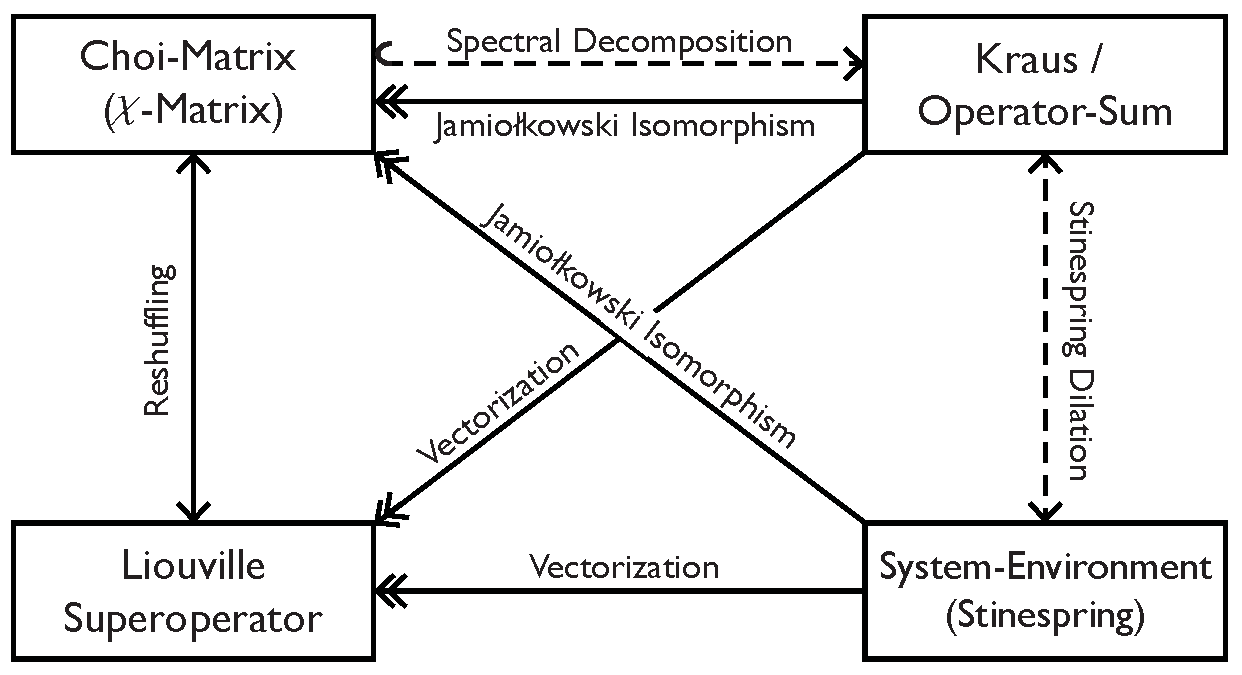
\includegraphics[width=13.5\xxxscale]{fig1}
%\caption{The main mathematical representations for completely positive maps and how one may transform between them. Solid arrows represent linear operations which we prove can be done by ``wire bending'' transformations in our graphical calculus. Dashed arrows represent non-linear transformations. Reshuffling and Stinespring dilation are bijective transformations, vectorization and the Jamio{\l}kowski isomorphism are surjective transformations, and the spectral decomposition is an injective transformation.}
\label{fig:cpreps}
\end{center}

\begin{remark}
In this chapter we will use the notation that $\2 X, \2 Y, \2 Z$ are finite-dimensional complex Hilbert spaces,  
 
 % PS
% \marginpar{HERE!}
%\begin{enumerate}
\begin{itemize}
\item[1.] % PS
${\mathcal L}(\2X,\2Y)$ is the space of bounded linear operators $A: \2 X\rightarrow \2 Y$ (with ${\mathcal L}(\2X)\equiv {\mathcal L}(\2X,\2X)$),
 %   
\item[2.]  %PS
$T(\2X,\2Y)$ is the space of operator maps $\2 E:{\mathcal L}(\2X)\rightarrow {\mathcal L}(\2Y)$  (with $T(\2X)\equiv T(\2X,\2X)$),
 \item[3.] and $C(\2X,\2Y)$ is the space of operator maps $\2 E$ which are CP.
%\end{enumerate}
\end{itemize}

\end{remark} % PS

    



\section{Kraus / Operator-Sum Representation}
\label{sec:kraus}

The first representation of CPTP-maps we cast into our framework is the \emph{Kraus}~\cite{Kraus1983} or \emph{operator-sum}~\cite{NC} representation. This representation is particularly useful in phenomenological models of noise in quantum systems.
\begin{theorem}
Kraus's theorem states that a linear map $\2 E\in T(\2X,\2Y)$ is CPTP if and only if it may be written in the form
\begin{equation}
\2 E(\rho)= \sum_{\alpha=1}^D K_\alpha \rho K_\alpha^\dagger
\label{eqn:kraus}
\end{equation}
where the Kraus operators $\{K_\alpha: \alpha=1,...,D\}$, $K_\alpha\in \Lx{X,Y}$, satisfy the completeness relation 
\begin{equation}
\sum_{\alpha=1}^D K_\alpha^\dagger K_\alpha = \I_{\2 X}.
\label{eqn:completeness}
\end{equation} 
\end{theorem}

The Kraus representation of $\2E$ in \eqref{eqn:kraus} has the graphical representation 
% FIGURE - KRAUS
\begin{center}
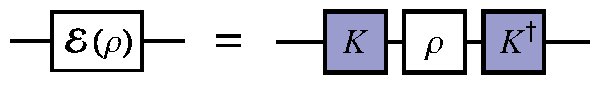
\includegraphics[width=0.6\textwidth]{fig23}
\label{fig:kraus-evo}
\end{center}

The maximum number of Kraus operators needed for a Kraus description of $\2 E$ is equal to the dimension of ${\mathcal L}(\2X,\2Y)$. For the case where $\2 X\cong\2 Y\cong\C^d$ the maximum number of Kraus operators is $d^2$, and the minimum number case corresponds to unitary evolution where there is only a single Kraus operator.

It is important to note that the Kraus representation of $\2 E$ is not unique as there is unitary freedom in choosing the Kraus operators. We can give preference to a particular representation called the \emph{Canonical Kraus Representation}~\cite{Bengtsson2006} which is the unique set of Kraus operators satisfying the orthogonality relation $\Tr[K^\dagger_\alpha K_\beta]=\lambda_\alpha\delta_{\alpha\beta}$. The canonical Kraus representation will be important when transforming between representations in \S~\ref{sec:trans}.


\section{System-Environment / Stinespring Representation}
\label{sec:se}

The second representation of CPTP-maps we consider is the system-environment model~\cite{NC}, which is typically considered the most physically intuitive description of open system evolution. This representation is closely related to (and sometimes referred to as) the Stinespring representation as it can be thought of as an application of the Stinespring dilation theorem~\cite{Stinespring1955}, which we also describe in this section.
\begin{theorem}
In this model, we consider a system of interest $\2 X$, called the \emph{principle system}, coupled to an additional system $\2 Z$ called the \emph{environment}. The composite system of the principle system and environment is then treated as a closed quantum system which evolves unitarily. We recover the reduced dynamics on the principle system by performing a partial trace over the environment. Suppose the initial state of our composite system is given by $\rho\otimes\tau \in {\mathcal L}(\2X\otimes\2Z)$, where $\tau\in {\mathcal L}(\2Z)$ is the initial state of the environment. The joint evolution is described by a unitary operator $U\in {\mathcal L}(\2X\otimes\2Z)$ and the reduced evolution of the principle system's state $\rho$ is given by
\begin{equation}
\2 E(\rho) = \Tr_{\2 Z}[U(\rho\otimes\tau)U^\dagger]
\label{eqn:sys-env}
\end{equation}
\end{theorem}

For convenience we can assume that the environment starts in a pure state $\tau=\ketbra{v_0}{v_0}$, and in practice one only need consider the case where the Hilbert space describing the environment has at most dimension $d^2$ for $\2 X\cong\C^d$~\cite{NC}. The system-environment representation of the CP-map $\2 E$ may then be represented graphically as 
% FIGURE - SE
\begin{center}
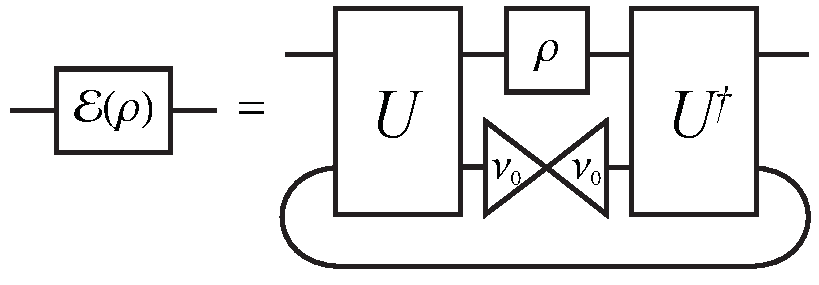
\includegraphics[width=0.52\textwidth]{fig24}
\label{fig:sys-env}   
\end{center}


The system-environment model is advantageous when modelling the environment as a physical system. However, care must be taken when ascribing physical reality to any particular model as the system-environment description is not unique. This is not surprising as many different physical interactions could give rise to the same reduced dynamics on the principle system. This freedom manifests in an ability to choose the initial state of the environment in the representation and then adjust the unitary operator accordingly. In practice, the system-environment model can be cumbersome for performing many calculations where the explicit dynamics of the environment system are irrelevant. The remaining descriptions, which we cast into diagrammatic form, may be more convenient in these contexts.

Note that the system-environment evolution for the most general case will be an isometry and this is captured in Stinespring's representation~\cite{Stinespring1955}.

\begin{theorem}
Stinespring's dilation theorem states that a CP-map $\2 E\in C(\2X,\2Y)$ can be written in the form
\begin{equation}
\2 E(\rho) = \Tr_Z\left[A\rho A^\dagger\right]
\label{eqn:stinespring}
\end{equation}
where $A\in {\mathcal L}(\2X,\2Y\otimes\2Z)$ and the Hilbert space $\2 Z$ has dimension at most equal to ${\mathcal L}(\2X,\2Y)$. Further, the map $\2 E$ is trace preserving if and only if $A^\dagger A=\I_{\2 X}$ ~\cite{Stinespring1955}.
\end{theorem}

In the case where $\2 Y\cong\2 X$, the Hilbert space $\XZ$ mapped into by the Stinespring operator $A$ is equivalent to the joint system-environment space in the system-environment representation. Hence one may move from the system-environment description to the Stinespring representation as follows:
% FIGURE - STINESPRING
\begin{center}
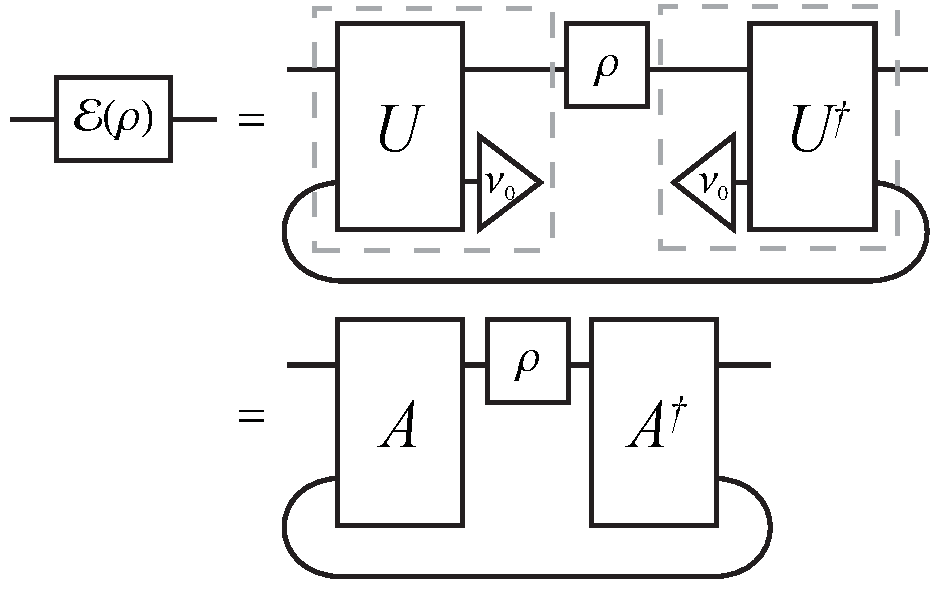
\includegraphics[width=0.55\textwidth]{fig25}
\label{fig:stinespring}
\end{center}
where $\ket{v_0}\in\2 Z$ is the initial state of the environment, and we have defined the Stinespring operator
\begin{equation}
A = U\cdot(\I_{\2 X}\otimes\ket{v_0}),\label{eqn:stinespring-se}.
\end{equation}

This close relationship is why these two representations are often referred to by the same name, and as we will show in \S~\ref{sec:to-se}, it is straight forward to construct a Stinespring representation from the Kraus representation. However, generating a full description of the joint system-environment unitary operator $U$ from a Stinespring operator $A$ is cumbersome. It involves an algorithmic completion of the matrix elements in the unitary $U$ not contained within the subspace of the initial state of the environment~\cite{Bengtsson2006}. Since it usually suffices to define the action of $U$ when restricted to the initial state of the environment, which by \eqref{eqn:stinespring-se} is the Stinepsring representation, this is often the only transformation one need consider.

\begin{remark}
A further important point is that the evolution of the principle system $\2 E(\rho)$ is guaranteed to be CP if and only if the initial state of the system and environment is separable; $\rho_{\2 X\2 Z}=\rho_{\2X}\otimes\rho_{\3 Z}$. In the case where the physical system is initially correlated with the environment, it is possible to have reduced dynamics which are non-completely positive~\cite{Weinstein2004,Carteret2008}, however such situations are beyond the scope of this chapter.  
\end{remark}

\section{Louiville-Superoperator Representation}
\label{sec:sop}

We now move to the \emph{linear superoperator} or \emph{Liouville} representation of a CP-map $\2 E\in C(\2X,\2Y)$. \begin{definition}
The superoperator representation is based on the vectorization of the density matrix $\rho \mapsto \dket{\rho}_\sigma$ with respect to some orthonormal operator basis $\{\sigma_\alpha : \alpha=0,...,d^2-1\}$ as introduced in \S~\ref{sec:vec}. Once we have chosen a vectorization basis (col-vec in our case) we define the superoperator for a map $\2 E\in T(\2X,\2Y)$ to be the linear map 
\begin{equation}
\2 S:\2X\otimes\2X\rightarrow\2Y\otimes\2Y: \dket{\rho}\mapsto \dket{\2 E(\rho)}	\label{eqn:sop}
\end{equation}


This is depicted graphically as
 %FIGURE - SUPEROP
 \begin{center}
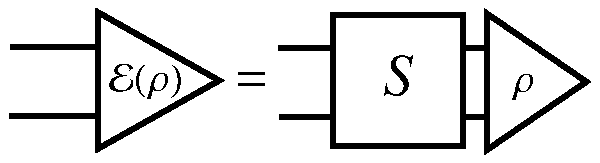
\includegraphics[width=0.4\textwidth]{fig26}
\label{fig:superop}     
\end{center}

 
 In the col-vec basis we can express the evolution of a state $\rho$ in terms of tensor components of $\2 S$ as
\begin{eqnarray}
\2 E(\rho)_{mn} &=& \sum_{\mu\nu} \2S_{nm,\nu\mu} \rho_{\mu\nu}.
\end{eqnarray}
\end{definition}
For the case where $\2 E \in T(\2X)$, it is sometimes  useful to change the basis of our superoperators from the col-vec basis to an orthonormal operator basis $\{\sigma_\alpha\}$ for ${\mathcal L}(\2X)$. This is done using the basis transformation operator $T_{c\rightarrow\sigma}$ introduced in \S~\ref{sec:vec}. We have
\begin{eqnarray}
\2 S_\sigma 
	&=& T_{c\rightarrow\sigma}\cdot \2 S \cdot T_{c\rightarrow\sigma}^\dagger \label{eqn:sop-basis-change}\\
	&=& \sum_{\alpha\beta} \2 S_{\alpha\beta} \,\dket{\sigma_\alpha}\dbra{\sigma_\beta}.
\end{eqnarray}
where the subscript $\sigma$ indicates that $\2 S_\sigma$ is the superoperator in the $\sigma$-vec convention. The tensor networks for this transformation is given by
% FIGURE - BASIS CHANGE
\begin{center}
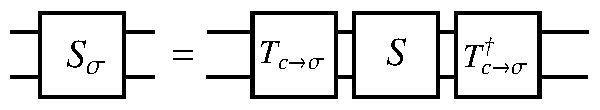
\includegraphics[width=0.5\textwidth]{fig27}  \label{fig:sop-change-basis}
\end{center}
\begin{remark}
For a general map $\2 E\in T(\2X,\2Y)$ we could do a similar construction but would need different bases for the initial and final Hilbert spaces ${\mathcal L}(\2X)$ and ${\mathcal L}(\2Y)$.
\end{remark}

The structural properties the superoperator $\2 S$ must satisfy for the linear map $\2 E$ to be hermitian-preserving (HP), trace-preserving (TP), and completely positive (CP) are~\cite{Bengtsson2006}:
\begin{eqnarray}
% SOP - HP
\2 E \mbox{ is HP } 
	&\Longleftrightarrow&  \overline{\2 S}=\2 S^S \label{eqn:sop-hpres}\hspace{10em}\\
	&\Longleftrightarrow&
	% FIGURE
	\parbox[c]{1em}{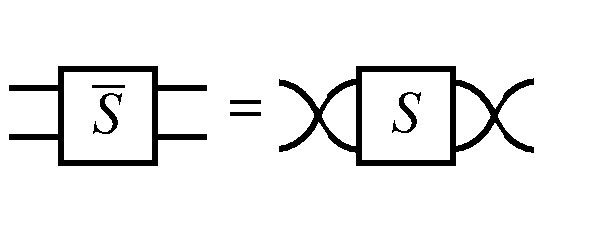
\includegraphics[width=0.28\textwidth, trim= 0cm 1cm 0cm 1cm,clip]{inline-fig1}}\\
% SOP - TP
\2 E \mbox{ is TP } 
	&\Longleftrightarrow&\2 S_{mm,n\nu}=\delta_{n\nu}\\
	&\Longleftrightarrow&
	% FIGURE
	\parbox[c]{1em}{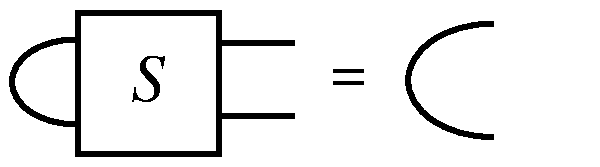
\includegraphics[width=0.2\textwidth]{inline-fig2}}\\
% SOP - CP
\2 E \mbox{ is CP } 
	&\Longleftrightarrow&\2 S_{\2 I\otimes \2 E}\dket{\rho_{AB}}\ge 0 ~\forall \rho_{AB}\ge0
\end{eqnarray}
\begin{remark}
There is not a convenient structural criteria on the superoperator $\2 S$ which specifies if $\2 E$ is a CP-map. To test for positivity or complete positivity one generally uses the closely related \emph{Choi-matrix} representation.
\end{remark}


Superoperators are convenient to use for many practical calculations. Unlike the system-environment model the superoperator $S$ is unique with respect to the choice of vectorization basis. Choosing an appropriate basis to express the superoperator in can often expose certain information about a quantum system. For example, if we want to model correlated noise for a mutli-partite system we can vectorize with respect to the mutli-qubit Pauli basis. Correlated noise would then manifest as non-zero entries in the superoperator corresponding to terms such as $\sigma_x\otimes\sigma_x$. 
We discus in more detail how this may be done in \S~\ref{sec:comp-sop}.





\section{Choi-Matrix Representation}
\label{sec:choi}

The final representation shown in Fig.~\ref{fig:cpreps} is the \emph{Choi matrix}~\cite{Choi1975}, or dynamical matrix~\cite{Bengtsson2006}. This is an application of the Choi-Jamio{\l}kowski isomorphism which gives a bijection between linear maps and linear operators~\cite{Jamiolkowski1972}.
\begin{definition}
Similarly to how vectorization mapped linear operators in ${\mathcal L}(\2X,\2Y)$ to vectors in $\XY$ or $\YX$, the Choi-Jamio{\l}kowski isomorphism maps linear operators in $T(\2X,\2Y)$ to linear operators in ${\mathcal L}(\2X\otimes\2Y)$ or ${\mathcal L}(\2Y\otimes\2X)$. 
The two conventions are
\begin{eqnarray}
\mbox{col-}\Lambda&:& 
	T(\2X,\2Y)\rightarrow {\mathcal L}(\2X\otimes\2Y):\,\, \2 E\mapsto \Lambda_c\\
\mbox{row-}\Lambda&:& 
	T(\2X,\2Y)\rightarrow {\mathcal L}(\2Y\otimes\2X):\,\, \2 E\mapsto \Lambda_r.
\end{eqnarray}
For $\2 X\cong\C^d$, the explicit construction of the Choi-matrix is given by
\begin{eqnarray} 
	\label{eqn:col-choi}
	\Lambda_c &=& \sum_{i,j=0}^{d-1}
	 \ketbra{i}{j}\otimes\2 E(\ketbra{i}{j})\\
	\Lambda_r &=& \sum_{i,j=0}^{d-1}
	 \2 E(\ketbra{i}{j})\otimes\ketbra{i}{j}
\end{eqnarray}
where $\{\ket{i}:i=0,\hdots,d-1\}$ is an orthonormal basis for $\2 X$.

\end{definition}



We call the two conventions col-$\Lambda$ and row-$\Lambda$ due to their relationship with the vectorization conventions introduced in \S~\ref{sec:vec}. 
\begin{definition}
The Choi-Jamio{\l}kowski isomorphism can also be thought of as having a map $\2 E\in T(\2X,\2Y)$ act on one half of an unnormalized Bell-state $\ket{\Phi^+}=\sum_i \ket{i}\otimes\ket{i} \in \2X\otimes\2X$, and hence these conventions corresponding to which half of the Bell state it acts on:
\begin{eqnarray} 
	\Lambda_c &=& (\2 I \otimes \2 E)\ketbra{\Phi^+}{\Phi^+}\label{eqn:jamiolkowski}\\
	\Lambda_r &=& (\2 E \otimes \2 I)\ketbra{\Phi^+}{\Phi^+}
\end{eqnarray}
where $\2 I\in T(\2X)$ is the identity map. 
\end{definition}

In what follows we will use the col-$\Lambda$ convention and drop the subscript from $\Lambda_c$. We note that the alternative row-$\Lambda$ Choi-matrix is naturally obtained by applying the bipartite-SWAP operation to $\Lambda_c$. 

As will be considered in \S~\ref{sec:to-choi}, if the evolution of the CP map $\2 E$ is described by a Kraus representation $\{K_i\}$, then the Choi-Jamio{\l}kowski isomorphism states that we construct the Choi-matrix by acting on one half of a bell state with the Kraus map as shown:

\begin{center}
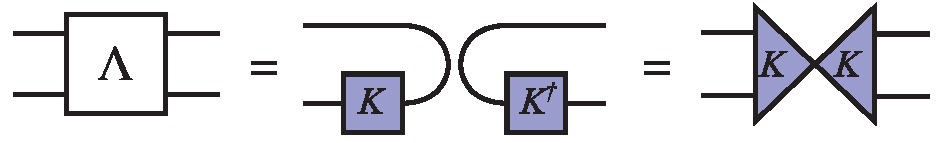
\includegraphics[width=0.7\textwidth]{fig28alt}
\label{fig:choi-jamiolkowski}
\end{center}

\begin{remark}
Note that in general any tensor network describing a linear map $\2 E$, not just the Kraus description, may be contracted with one-half of the maximally entangled state $\ketbra{\Phi^+}{\Phi^+}$ to construct the Choi-matrix.
\end{remark}

With the Choi-Jamio{\l}kowski isomorphism defined, the evolution of a quantum state in terms of the Choi-matrix is then given by
\begin{eqnarray}
\2 E(\rho) &=& \Tr_{\2 X} \left[ (\rho^T\otimes \I_{\2 Y} )\Lambda \right]
\label{eqn:choi-evo}
\end{eqnarray}
or in terms of tensor components
\begin{eqnarray}
\2 E(\rho)_{mn}
		&=&\sum_{n,m} \Lambda_{\mu m,\nu n}\rho_{\mu\nu}.
\end{eqnarray}
%FIGURE - CHOI
The tensor network for \eqref{eqn:choi-evo} is given by
\begin{center}
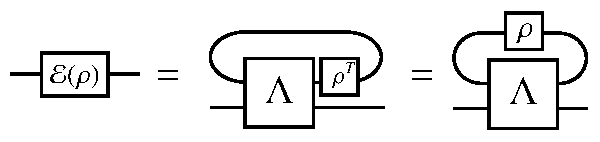
\includegraphics[width=0.6\textwidth]{fig29}
\label{fig:choi-evo}    
\end{center}
The graphical proof of \eqref{fig:choi-evo} for the case where $\2 E$ is described by a Kraus representation is as follows:
 %FIGURE - CHOI
 \begin{center}
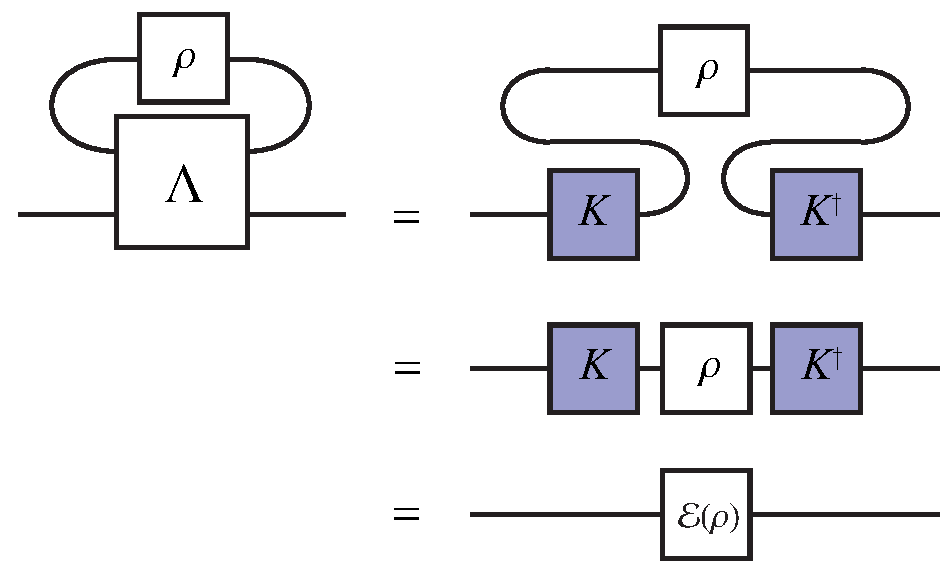
\includegraphics[width=0.6\textwidth]{fig30}\label{fig:choi-evo-proof}    
 \end{center}
\begin{remark}
The structural properties the Choi-matrix $\Lambda$ must satisfy for the linear map $\2 E$ to be hermitian-preserving (HP), trace-preserving (TP),  and completely positive (CP) are~\cite{Bengtsson2006}:
\begin{eqnarray}
% CHOI - HP
\2 E \mbox{ is HP } 
	&\Longleftrightarrow&  \Lambda^\dagger=\Lambda \label{eqn:choi-HP}\hspace{10em}\\
	&\Longleftrightarrow&
	% FIGURE
	\parbox[c]{1em}{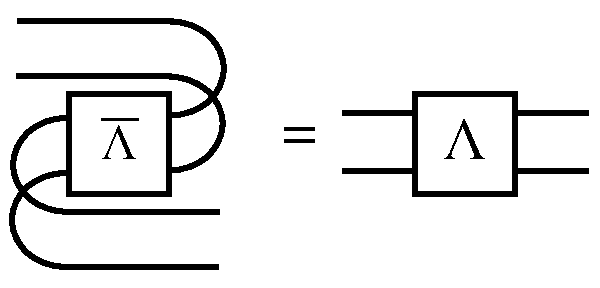
\includegraphics[width=0.3\textwidth]{inline-fig3}}\\
% CHOI - TP
\2 E \mbox{ is TP } 
	&\Longleftrightarrow& \Tr_{\2 Y}[\Lambda]=\I_{\2 X}\label{eqn:choi-TP}\\
	&\Longleftrightarrow&
	% FIGURE
	\parbox[c]{1em}{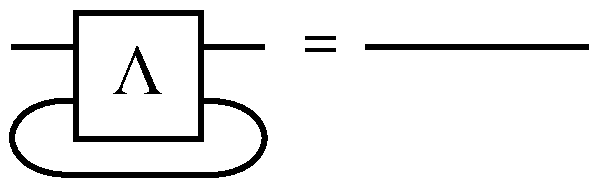
\includegraphics[width=0.3\textwidth]{inline-fig4}}\label{eqn:choi-tp}\\
% CHOI - CP
\2 E \mbox{ is CP } 
	&\Longleftrightarrow&  \Lambda\ge 0.\label{eqn:choithm}
\end{eqnarray}
\end{remark}



The Choi-matrix for a given map $\2 E$ is unique with respect to the isomorphism convention chosen. We will provide tensor networks to illustrate a close relationship to the superoperator formed with the corresponding vectorization convention in \S~\ref{sec:choi-sop}. The Choi-matrix finds practical utility as one can check the complete-positivity of the map $\2 E$ by computing the eigenvalues of $\Lambda$. It is also necessary to construct the Choi-matrix for a given superoperator to transform to the other representations. 

Due to the similarity of vectorization and the Choi-Jamio{\l}kowski isomorphism, one could then ask what happens if we vectorize in a different basis. This change of basis of the Choi-matrix is more commonly known as the $\chi$-matrix which we will discuss next. However, such a change of basis does not change the eigen-spectrum of a matrix, so the positivity criteria in \eqref{eqn:choithm} holds for any basis.

Another desirable property of Choi matrices is that they can be directly determined for a given system experimentally by \emph{ancilla assisted process tomography (AAPT)}~\cite{DAriano2003,White2003}. This is an experimental realization of the Choi-Jamio{\l}kowski isomorphism which we discuss in detail in \S~\ref{sec:aapt}.



\section{Process Matrix Representation}
\label{sec:chi}

As previously mentioned, one could consider a change of basis of the Choi-matrix analogous to that for the superoperator. The resulting operator is more commonly known as the \emph{$\chi$-matrix} or \emph{process matrix}~\cite{NC}.

\begin{definition}
Consider Hilbert spaces $\2 X\cong\C^{d_x}$, $\2 Y\cong\C^{d_y}$ and let $D=d_x d_y$, and $\2Z \cong \C^D$. If one chooses an orthonormal operator basis  $\{\sigma_\alpha: \alpha=0,...,D-1\}$ for ${\mathcal L}(\2X,\2Y)$, then a CPTP map $\2 E\in C(\2X,\2Y)$ may be expressed in terms of a matrix $\chi\in {\mathcal L}(\2Z)$ as
\begin{eqnarray}
\2 E(\rho)
&=&\sum_{\alpha,\beta=0}^{D-1} \chi_{\alpha\beta} \sigma_\alpha \rho \sigma_\beta^\dagger
\label{eqn:chi-evo}
\end{eqnarray}
where the process matrix $\chi$ is unique with respect to the choice of basis $\{\sigma_\alpha\}$.
\end{definition}
 

The process matrix with respect to an orthonormal operator basis $\{\sigma_\alpha\}$ is related to the Choi matrix by the change of basis
\begin{eqnarray}
\chi	&=& T_{c\rightarrow\sigma} \cdot \Lambda \cdot T^\dagger_{c\rightarrow\sigma}
\label{eqn:choi-to-chi}\\
\Rightarrow \Lambda&=& \sum_{\alpha,\beta} \chi_{\alpha\beta} \dketdbra{\sigma_\alpha}{\sigma_\beta}
\end{eqnarray}
where $T_{c\rightarrow\sigma}$ is the vectorization change of basis operator introduced in \S~\ref{sec:vec}. Thus evolution in terms of the $\chi$-matrix is analogous to our Choi evolution as shown below:
 %FIGURE - CHI EVO
\begin{center}
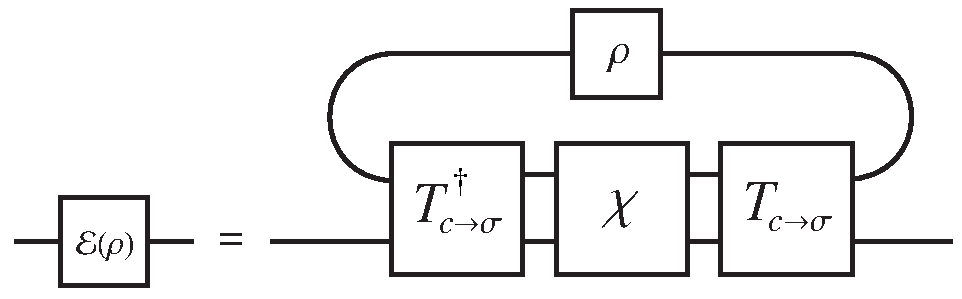
\includegraphics[width=0.5\textwidth]{fig31}
\label{fig:chi-evo}    
\end{center}

 %FIGURE - CHI PROOFS
Starting with the expression for process matrix evolution in \eqref{eqn:chi-evo}, the  graphical proof asserting the validity of \eqref{eqn:choi-to-chi} is as follows
\begin{center}
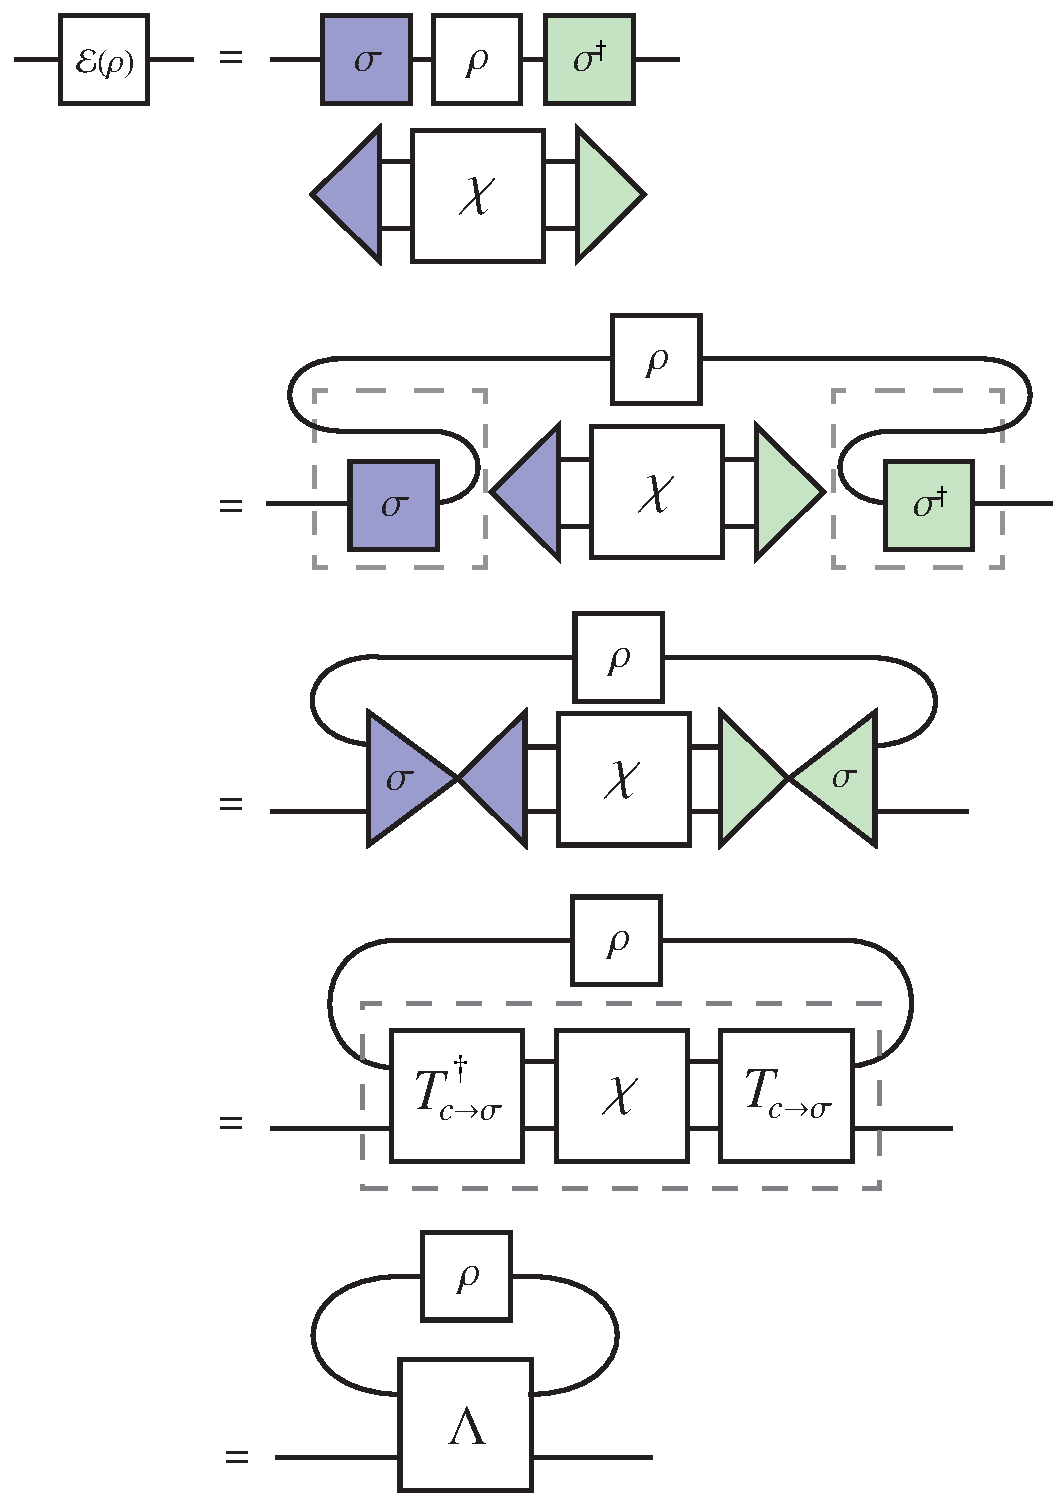
\includegraphics[width=0.55\textwidth]{fig32} \label{fig:choi-to-chi}   
\end{center}

%
We also see that if one forms the process matrix with respect to the col-vec basis $\sigma_\alpha = E_{j,i}$ where $\alpha = i+dj$ and $d$ is the dimension of $\2 H$, then we have $\chi=\Lambda$. 
 


\begin{remark}
Since the process matrix is a unitary transformation of the Choi-matrix, it shares the same structural conditions for hermitian preservation and complete-positivity as for the Choi-matrix given in~\eqref{eqn:choi-HP} and \eqref{eqn:choithm} respectively.
The condition for it to be trace preserving may be written in terms of the matrix elements and basis however. These conditions are
\begin{eqnarray}
\2 E \mbox{ is TP} &\Longleftrightarrow&
\Tr_{\2 Y}\left[T^\dagger_{c\rightarrow\sigma}\chi T_{c\rightarrow\sigma}\right]=\I_{\2 X}\\
&\Longleftrightarrow& \sum_{\alpha,\beta} \chi_{\alpha,\beta} \sigma_{\alpha}^T \overline{\sigma}_\beta = \I_{\2 X}\\
\2 E \mbox{ is HP} &\Longleftrightarrow& \chi^\dagger=\chi\\
\2 E \mbox{ is CP} &\Longleftrightarrow& \chi\ge0.
\end{eqnarray}
\end{remark}


To convert a process-matrix $\chi$ in a basis $\{\sigma_\alpha\}$ to another orthonormal operator basis $\{\omega_\alpha\}$, we may use the same change of basis transformation as used for the superoperator change of basis in \S~\ref{sec:sop}. That is
\begin{eqnarray}
\chi^\omega	&=& T_{\sigma\rightarrow\omega} \cdot \chi^\sigma \cdot T^\dagger_{\sigma\rightarrow\omega}\\
		&=& \sum_{\alpha\beta} \chi^\sigma_{\alpha\beta}\,\, \dket{\sigma_\alpha}_\omega\dbra{\sigma_\beta}_\omega
\end{eqnarray}
where the superscripts $\sigma,\omega$ denote the basis of the $\chi$-matries. This is illustrated as
%FIGURE - CHI BASIS CHANGE
\begin{center}
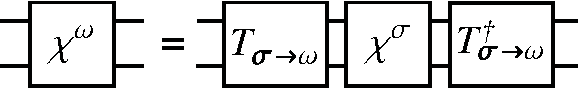
\includegraphics[width=0.45\textwidth]{fig33}  \label{fig:chi-change-basis}    
\end{center}


%%%%%%%%%%%%%%%%%%%%%%%%%%%%%%%%%%%%%%%%%%%%%%%%%%%%%%%%
\section{Transforming between representations}
\label{sec:trans}


\subsection{Transformations between the Choi-matrix and superoperator representations}
\label{sec:choi-sop}

The Choi-matrix and superoperator are naturally equivalent under the reshuffling wire bending duality introduced in \S~\ref{sec:bipartite}.  In the col (row) convention we may transform between the two by applying the bipartite col (row)-reshuffling operation $R$ introduced in \S~\ref{sec:bipartite}. Let $\Lambda\in \LXY$ be the Choi-matrix, and $\2 S\in \Lx{\XX,\YY}$ be the superoperator, for a map $\2 E\in \Tx{X,Y}$. Then we have
\begin{eqnarray}
\Lambda &=& \2S^{R} \quad\quad\2 S = \Lambda^{R}
\end{eqnarray}
The tensor networks for these transformations using the col convention are
%FIGURE - CHOI <-> SOP

\begin{center}
\begin{tabular}{c|c}
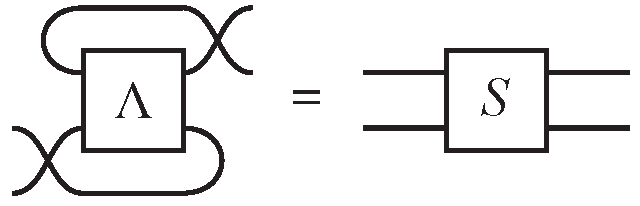
\includegraphics[width=.4\textwidth]{fig34a}
\hspace{2em} & \hspace{2em}
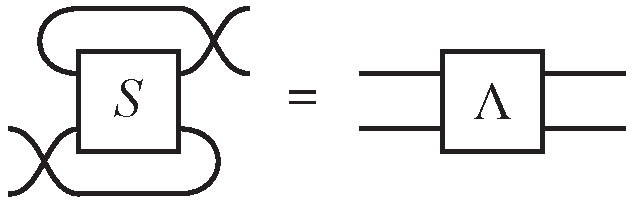
\includegraphics[width=.4\textwidth]{fig34b}
\end{tabular}
\label{fig:choi-sop}
\end{center}
In terms of tensor components we have
\begin{eqnarray}
\Lambda_{mn,\mu\nu} 	&=& \2 S_{\nu n,\mu m}
\end{eqnarray}
where $m,n$ and $\mu,\nu$ index the standard bases for $\2 X$ and $\2 Y$ respectively. Graphical proofs of the relations $\Lambda^{R_c}=\2 S$ and $\2 S^{R_c}=\Lambda$ are given below
% FIGURE - CHOI SOP PROOF

\begin{center}
\begin{tabular}{c|c}
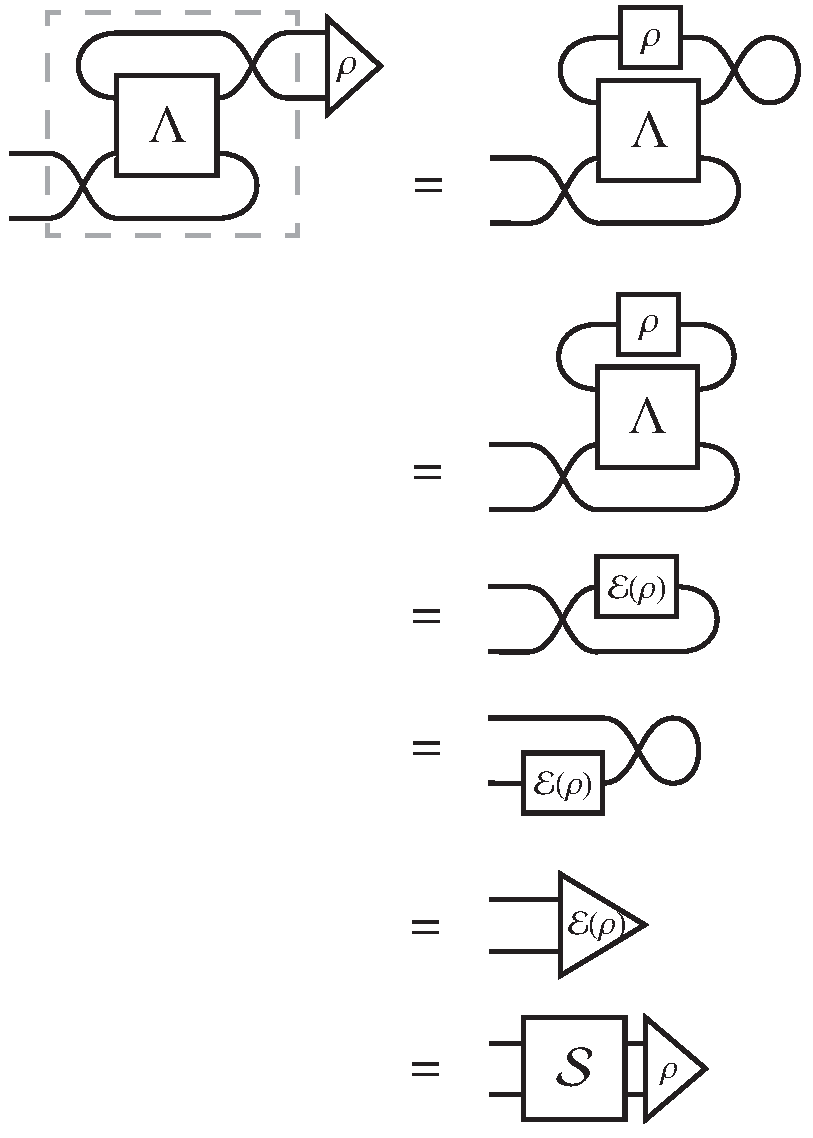
\includegraphics[width=0.4\textwidth]{fig35} 
\quad\quad&\quad
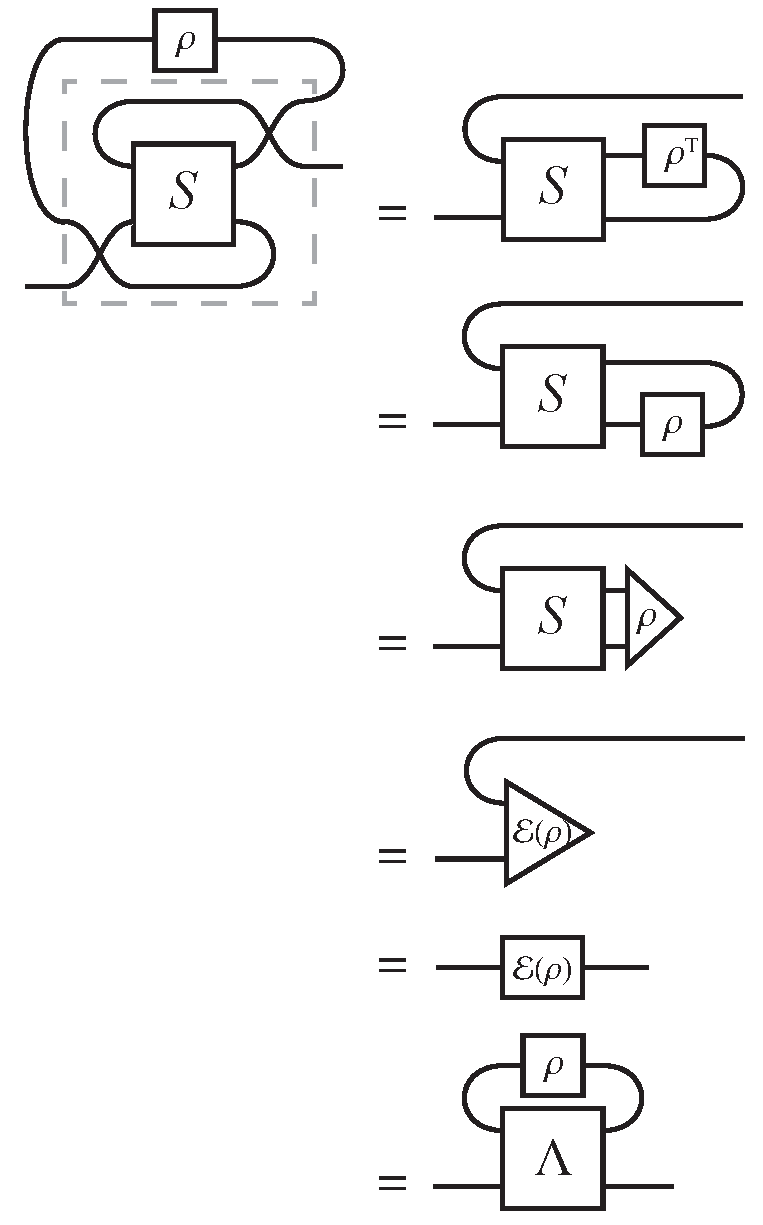
\includegraphics[width=0.4\textwidth]{fig36}
\end{tabular}
 \label{fig:choi-sop-proof}
\end{center}


\begin{remark}
To transfer between a $\chi$-matrix with respect to an arbitrary operator basis, and a superoperator with respect to an arbitrary vectorization basis, we must first convert both to col-vec (or row-vec) convention and then proceed by reshuffling.
\end{remark}
Note that reshuffling is its own inverse, i.e $(\Lambda^R)^R=\Lambda$, hence the solid bi-directional arrow connecting the Choi-matrix and superoperator representations in Fig.~\ref{fig:cpreps}. This is the only transformation between the representations we consider which is linear, bijective, and self-inverse.

%%%%%%%%%%%%%%%%%%%%%%%%%%%%%%%%%%%%%%%%%%%%%%%%%%%

\subsection{Transformations to the superoperator representation}
\label{sec:to-sop}

Transformations to the superoperator from the Kraus and system-environment representations of a CP-map are also accomplished by a wire-bending duality, in this case vectorization. However, unlike the bijective equivalence of the Choi-matrix and superoperator under the reshuffling duality, the vectorization duality is only surjective.

If we start with a Kraus representation for a CPTP map $\2 E\in\Cx{X,Y}$ given by $\{K_\alpha: \alpha=0,...,D-1 \}$, with $K_\alpha\in \Lx{X,Y}$, we can construct the superoperator $\2 S \in \Lx{\XX,\YY}$ by 
\begin{eqnarray}
\2 S &=&\sum_{\alpha=0}^{D-1} \overline{K}_\alpha\otimes K_\alpha.
\label{eqn:kraus-to-choi}
\end{eqnarray}
The corresponding tensor network is  
% FIGURE - KRAUS TO SOP
\begin{center}
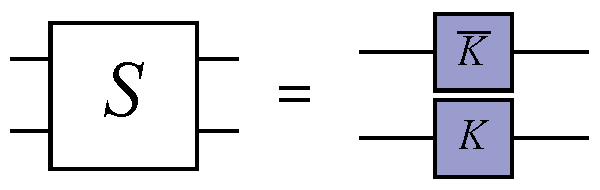
\includegraphics[width=0.35\textwidth]{fig37}
\label{fig:kraus-sop}
\end{center}
and the graphical proof of this relationship follows directly from Roth's lemma:
% FIGURE - KRAUS TO SOP PROOF
\begin{center}
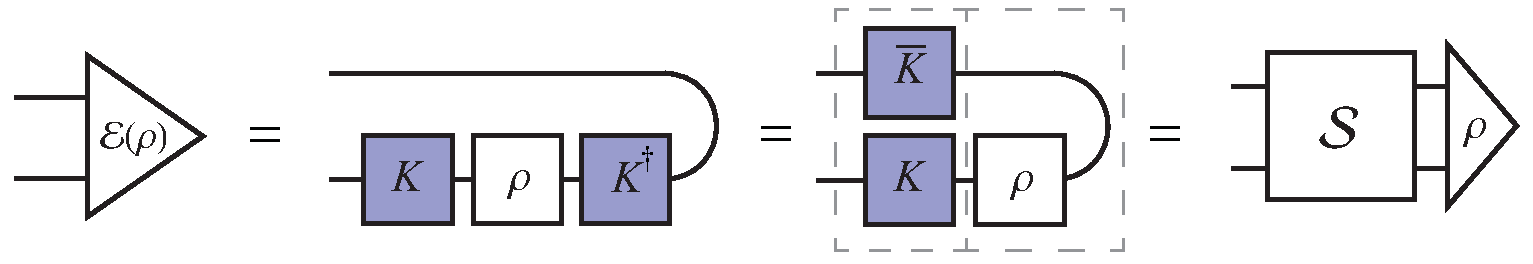
\includegraphics[width=0.9\textwidth]{fig38alt}
\label{fig:kraus-sop-proof}
\end{center}

Starting with a system-environment (or Stinespring) representation of a map $\2 E\in\Cx{X,Y}$ with input and output system Hilbert spaces $\2 X\cong \C^{d_x}$ and $\2Y\cong \C^{d_y}$ respectively, and environment Hilbert space $\2 Z\cong \C^D$ with $1\le D \le d_x d_y$, we may construct the superoperator for this map from the joint system-environment unitary $U$ and initial environment state $\ket{v_0}$ by
\begin{eqnarray}
\2 S &=& \sum_{\alpha} \bra{\alpha}\overline{U}\ket{v_0}\otimes \bra{\alpha}U\ket{v_0}, \label{eqn:se-to-sop}
\end{eqnarray}
where $\{\ket{\alpha}:\alpha=0,...,D-1\}$ is a real, orthonormal basis for $\2 Z$. The corresponding tensor network is 
\begin{center}
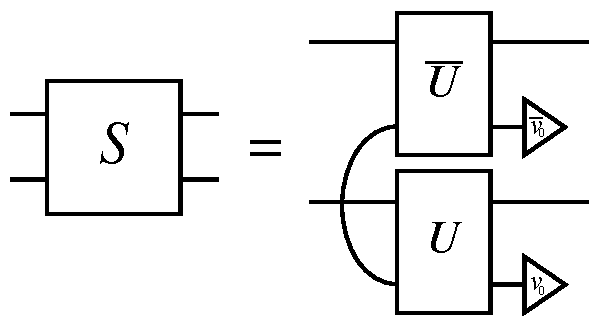
\includegraphics[width=0.35\textwidth]{fig39}
 \label{fig:se-sop}
\end{center}
 As with the Kraus to superoperator transformation, the proof of \eqref{eqn:se-to-sop} follows from Roth's lemma.

 
Note that while the vectorization wire bending duality is invertible, these transformations to the superoperator from the Kraus and system-environment representations are single directional. In both cases injectivity fails as the superoperator is unique, while both the Kraus and system-environment representations are not. Hence we have solid single directional arrows in Fig.~\ref{fig:cpreps} connecting both the Kraus and system-environment representations to the superoperator. The inverse transformation from a superoperator to the Kraus or system-environment representation requires a canonical decomposition of the operator $\2 S$ (via first reshuffling to the Choi-matrix), which is detailed in Sections~\ref{sec:to-kraus} and \ref{sec:to-se}.

%%%%%%%%%%%%%%%%%%%%%%%%%%%%%%%%%%%%%%%%%%%%%%%%%%%%%%%%

\subsection{Transformations to the Choi-matrix representation}
\label{sec:to-choi}

Transforming to the Choi-matrix from the Kraus and system-environment representations is accomplished via a wire-bending duality which captures the Choi-Jamio{\l}kowski isomorphism. As with the case of transforming to the superoperator, this duality transformation is surjective but not injective.

Given a set of Kraus matrices $\{ K_\alpha: \alpha=0,...,D-1\}$ where $K_\alpha\in\Lx{X,Y}$ for a CPTP-map $\2 E\in\Cx{X,Y}$, one may form the Choi-Matrix $\Lambda$ as was previously illustrated in \eqref{fig:choi-jamiolkowski} in \S~\ref{sec:choi}. In terms of both Dirac notation and tensor components we have:

\begin{eqnarray}
\Lambda	&=& \sum_{i,j}\left( \ketbra{i}{j}\otimes \sum_\alpha K_\alpha\ketbra{i}{j}K^\dagger_\alpha\right)\\
		&=& \sum_{\alpha} \dketdbra{K_\alpha}{K_\alpha}\\
\Lambda_{mn,\mu\nu}&=&\sum_\alpha (K_\alpha)_{\mu m}(\overline{K}_\alpha)_{\nu n}.
\end{eqnarray}
%TODO Page 127, Eq. (35.7): Are the indices at \Lambda in the right order?   As far as I understand, \Lambda is a density operator acting on X \otimes Y.  Shouldn't it be \Lambda_{m\mu,n\nu} instead of \Lambda_{mn,\mu\nu} ?
where $\{\ket{i}\}$ is an orthonormal basis for $\2 X$, $m,n$ index the standard basis for $\2 X$, and $\mu,\nu$ index the standard basis for $\2 Y$.

Given a system-environment representation with joint unitary $U\in \Lx{\XZ}$ and initial environment state $\ket{v_0}\in \2 Z$ we have
\begin{eqnarray}
\Lambda	&=&	\sum_{i,j}\left(\ketbra{i}{j}\otimes 
			\Tr_{\2 Z}\left[U\ketbra{i}{j}\otimes\ketbra{v_0}{v_0}U^\dagger\right]\right)
\end{eqnarray}
Graphically this is given by
% FIGURE - CHOI - STINESPRING
\begin{center}
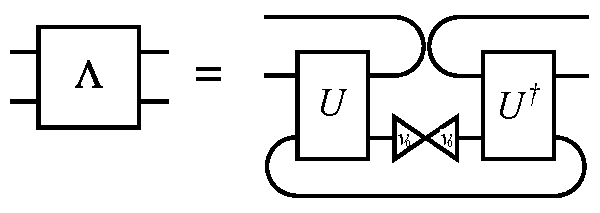
\includegraphics[width=0.4\textwidth]{fig40}
\label{fig:choi-se}
 \end{center}
The proof of these transformations follow directly from the definition of the Choi-matrix in \eqref{eqn:col-choi}, and the tensor networks for the evolution via the Kraus or system-environment representations given in \eqref{fig:kraus-evo} and \eqref{fig:sys-env} respectively. As with the vectorization transformation to the superoperator discussed in \S~\ref{sec:to-sop}, even though the Choi-Jamio{\l}kowski isomorphism is linear these transformations are single directional as injectivity fails due to the non-uniqueness of both the Kraus and system-environment representations. Hence we have the solid single-directional arrows connecting both the Kraus and system-environment representations to the Choi-matrix in Fig.~\ref{fig:cpreps}. 
 
This completes our description of the linear transformations between the representations of CP-maps in Fig.~\ref{fig:cpreps}. We will now detail the non-linear transformations to the Kraus and system environment representations. 

%%%%%%%%%%%%%%%%%%%%%%%%%%%%%%%%%%%%%%%%%%%%%%%%%%%%%

\subsection{Transformations to the Kraus Representation}
\label{sec:to-kraus}

We may construct a Kraus representations from the Choi matrix or system environment representation by the non-linear operations of spectral-decomposition and partial trace decomposition respectively. To construct a Kraus representation from the Superoperator however, we must first reshuffle to the Choi matrix. 

To construct Kraus matrices from a Choi matrix we first recall the graphical Spectral decomposition we introduced as an example of our color summation convention. If  $\2 E$ is CP, by \eqref{eqn:choithm} we have $\Lambda\ge0$ and hence the spectral decomposition of the Choi-matrix is given by
\begin{equation}
\Lambda=\sum_\alpha \mu_\alpha \ketbra{\phi_\alpha}{\phi_\alpha}, 
\end{equation}
where  $\mu_\alpha \ge 0$ are the eigenvalues, and $\ket{\phi_\alpha}$ the eigenvectors of $\Lambda$. Hence we can define Kraus operators $K_\alpha= \lambda_\alpha A_\alpha$ where $\lambda_\alpha = \sqrt{\mu_\alpha}$ and $A_\alpha$ is the unique operator satisfying $\dket{A_\alpha}=\ket{\phi_\alpha}$ as illustrated: 
% FIGURE - CHOI 2 KRAUS
\begin{center}
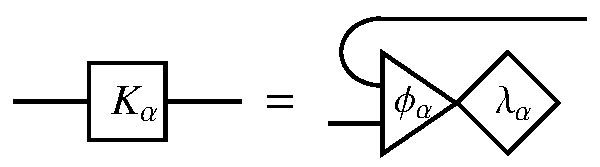
\includegraphics[width=0.35\textwidth]{fig41}
\label{fig:choi2kraus}
\end{center}
The number of Kraus operators will be equal to the rank $r$ of the Choi matrix, where $1\le r\le \mbox{dim}(\Lx{X,Y})$. The graphical proof of this transformation is as follows:
 % FIGURE - CHOI TO KRAUS PROOF
 \begin{center}
 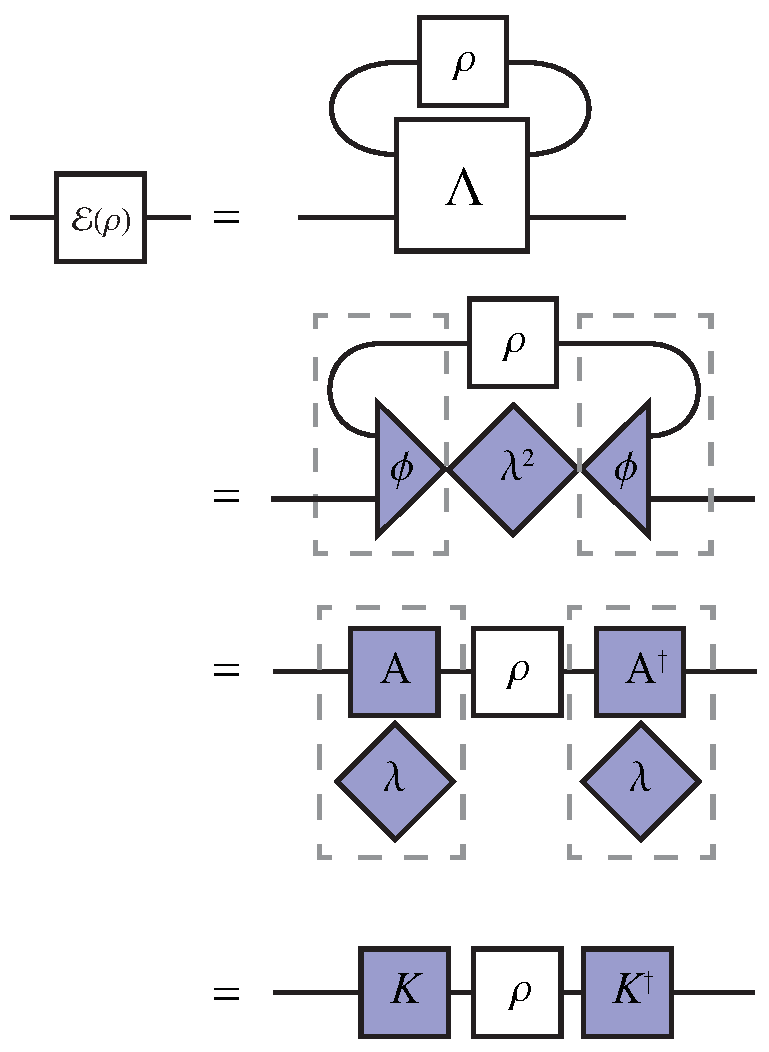
\includegraphics[width=0.42\textwidth]{fig42} \label{fig:choi-kraus-proof}
 \end{center}
The proof that Kraus operators satisfy the completeness relation follows from the trace preserving property of $\Lambda$ in \eqref{eqn:choi-TP}: 
\begin{center}
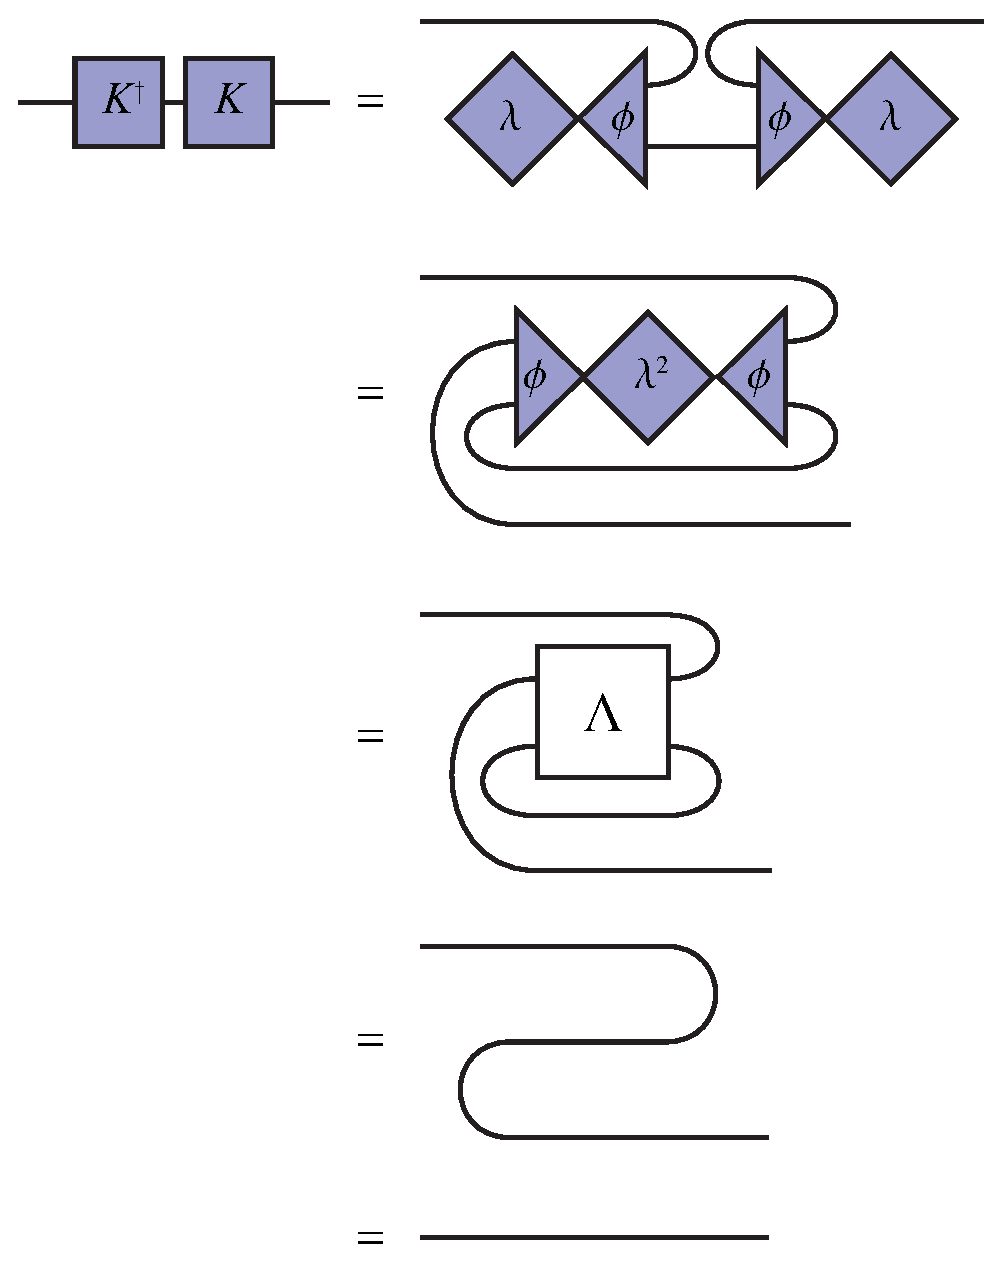
\includegraphics[width=0.43\textwidth]{fig43}
\label{fig:completeness-proof}
\end{center}
Note that since $\Lambda$, and the $\chi$-matrix are related by a unitary change of basis, the Kraus representations constructed from their respective spectral decompositions will also be related by the same transformation. Each will give a unitarily equivalent Canonical Kraus representation of $\2 E$ since the eigen-vectors are orthogonal. Thus we have described the arrow in Fig.~\ref{fig:cpreps} connecting the Choi matrix to the Kraus representation. It is represented as a dashed arrow as it involves a non-linear decomposition, and is single directional as this representation transformation is injective, but not surjective. Surjectivity fails as we can only construct the canonical Kraus representations for $\2 E$. The reverse transformation is given by the Jamio{\l}kowski isomorphism described in \S~\ref{sec:to-choi}.

Starting with a system-environment representation with joint unitary $U\in \Lx{\XZ}$ and initial environment state $\ket{v_0}\in\2 Z$, we first choose an orthonormal basis $\{\ket{\alpha}:\alpha=0,...,D-1\}$ for $\2 Z$. We then construct the Kraus representation by decomposing the partial trace in this basis as follows
\begin{eqnarray}
\2 E(\rho) 
	&=&\Tr_E\left[U\left(\rho\otimes\ketbra{v}{v}\right)U^\dagger\right] \\
	&=& \sum_{\alpha=0}^{D-1} \bra{\alpha}U\ket{v_0} \rho \bra{v_0}U^\dagger\ket{\alpha}\\
	&=& \sum_{\alpha=0}^{D-1} K_\alpha \rho K_\alpha^\dagger.
\end{eqnarray}
Hence we may define Kraus matrices 
\begin{equation}
K_\alpha = \bra{\alpha}U\ket{v_0}
\label{eqn:kraus-se-proof}
\end{equation}
 leading to the tensor network 
 % FIGURE - SE TO KRAUS
 \begin{center}
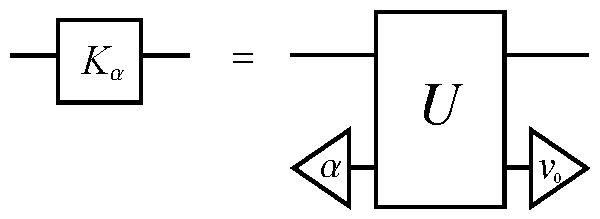
\includegraphics[width=0.35\textwidth]{fig44} \label{fig:kraus-sys-env}
 \end{center}
The graphical proof of \eqref{eqn:kraus-se-proof} and \eqref{fig:kraus-sys-env} is as follows
 % FIGURE - SE TO KRAUS PROOF
\begin{center}
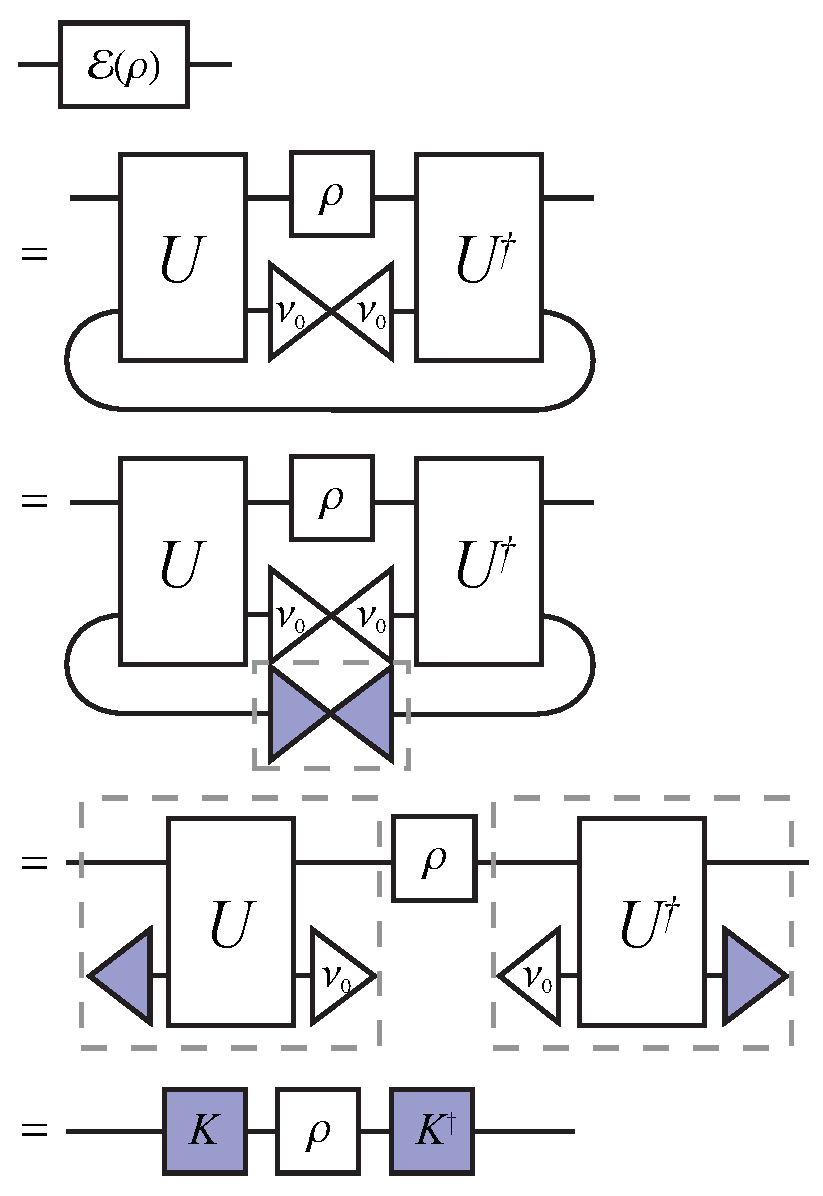
\includegraphics[width=0.45\textwidth]{fig45} 
\label{fig:kraus-sys-env-proof}
\end{center}
 
Though the Kraus and system-environment representations are both non-unique, for a fixed environment basis this partial trace decomposition is an injective transformation between the Kraus and Stinespring representations (or equivalently between the Kraus and system-environment representations when the joint unitary is restricted to a fixed initial state of the environment). 
To see this  let $\{K_\alpha\}$ and $\{J_\alpha\}$ be two Kraus representations for a CPTP-map $\2 E\in\Cx{X,Y}$, constructed from Stinespring representations $A$ and $B$ respectively. We have that
\begin{eqnarray}
K_\alpha &=& J_\alpha\\
&\Leftrightarrow& (K_\alpha)_{ij}= (J_\alpha)_{ij}\\
&\Leftrightarrow& A_{i\alpha,j} = B_{i\alpha,j}\\
&\Leftrightarrow& A=B.
\end{eqnarray}
Since the Stinespring operators satisfy $A=U\ket{v_0}$ and $B=V\ket{v_0}$ for some joint unitaries $U$ and $V$, we must have that $U_0=V_0$ where $U_0$ and $V_0$ are the joint unitaries restricted to the subspace of the environment spanned by $\ket{v_0}$.

This transformation can be thought of as the reverse application of the Stinespring dilation theorem, and hence for a fixed choice of basis (and initial state of the environment) it is invertible. The inverse transformation is the Stinespring dilation, and as we will show in \S~\ref{sec:to-se}, since the inverse transformation is also injective this transformation is a bijection. However, since the partial trace decomposition involves a choice of basis for the environment it is non-linear --- hence we use a dashed bi-directional arrow to represent the transformation from the system-environment representation to the Kraus representation in Fig.~\ref{fig:cpreps}. 

%%%%%%%%%%%%%%%%%%%%%%%%%%%%%%%%%%%%%%%%%%%%%%%%%%

\subsection{Transformations to the system-environment representation}
\label{sec:to-se}

We now describe the final remaining transformation given in Fig.~\ref{fig:cpreps}, the bijective non-linear transformation from the Kraus representation to the system-environment, or Stinespring, representation. The system-environment representation is the most cumbersome to transform to as it involves the unitary competition of a Stinespring dilation of a Kraus representation. Thus starting from a superoperator one must first reshuffle to the Choi-matrix, then from the Choi-matrix description one must then spectral decompose to the canonical Kraus representation, before finally constructing the system-environment as follows.

Let $\{ K_\alpha:\alpha=0,..., D-1\}$, where $1\le D\le \mbox{dim}(\Lx{X,Y})$, be a Kraus representation for the CP-map $\2 E\in \Tx{X,Y}$. Consider an ancilla Hilbert space $\2 Z\cong \C^D$, this will model the environment. If we choose an orthonormal basis for the environment, $\{\ket{\alpha}: \alpha=0,...,D-1\}$, then by Stinesprings dilation theorem we may construct the Stinespring matrix for the CP map $\2 E$ by 
\begin{equation}
A = \sum_{\alpha=0}^{D-1} K_\alpha \otimes\ket{\alpha}.
\label{eqn:kraus2stinespring}
\end{equation}

Recall from \S~\ref{sec:se} that the Stinespring representation is essentially the system-environment representation when the joint unitary operator is restricted to the subspace spanned by the initial state of the environment. Hence if we let $\ket{v_0}\in \2 Z$ be the initial state of the environment system, then this restricted unitary is given by
\begin{equation}
U_0 = \sum_\alpha K_\alpha\otimes\ketbra{\alpha}{v_0},\label{eqn:kraus-to-U}.
\end{equation} 
The tensor networks for \eqref{eqn:kraus2stinespring} and \eqref{eqn:kraus-to-U} are:
% FIGURE - STINESPRINE SE
\begin{center}
\begin{tabular}{c|c}
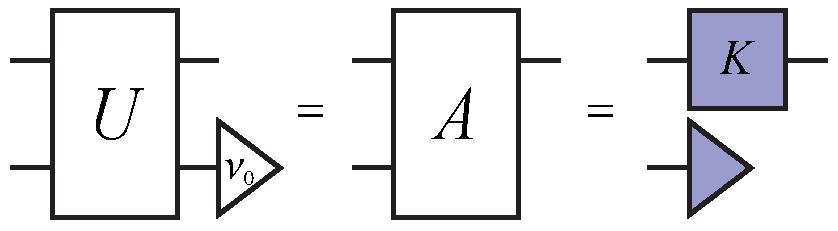
\includegraphics[width=0.42\textwidth]{fig46a}	
\quad\quad&\quad\quad
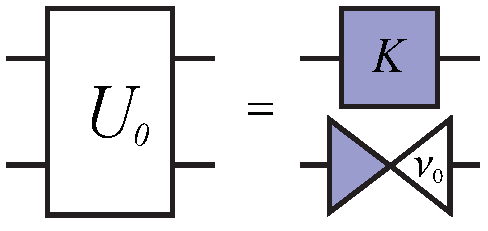
\includegraphics[width=0.25\textwidth]{fig46b}	\\
\footnotesize{(a) Stinespring operator}	&
\footnotesize{(a) Restricted unitary}
\end{tabular}
 \label{fig:sys-env-kraus}
\end{center}
%
The graphical proof that this construction gives the required evolution of a state $\rho$ is as follows
% FIGURE - STINESPRINE SE PROOF
\begin{center}
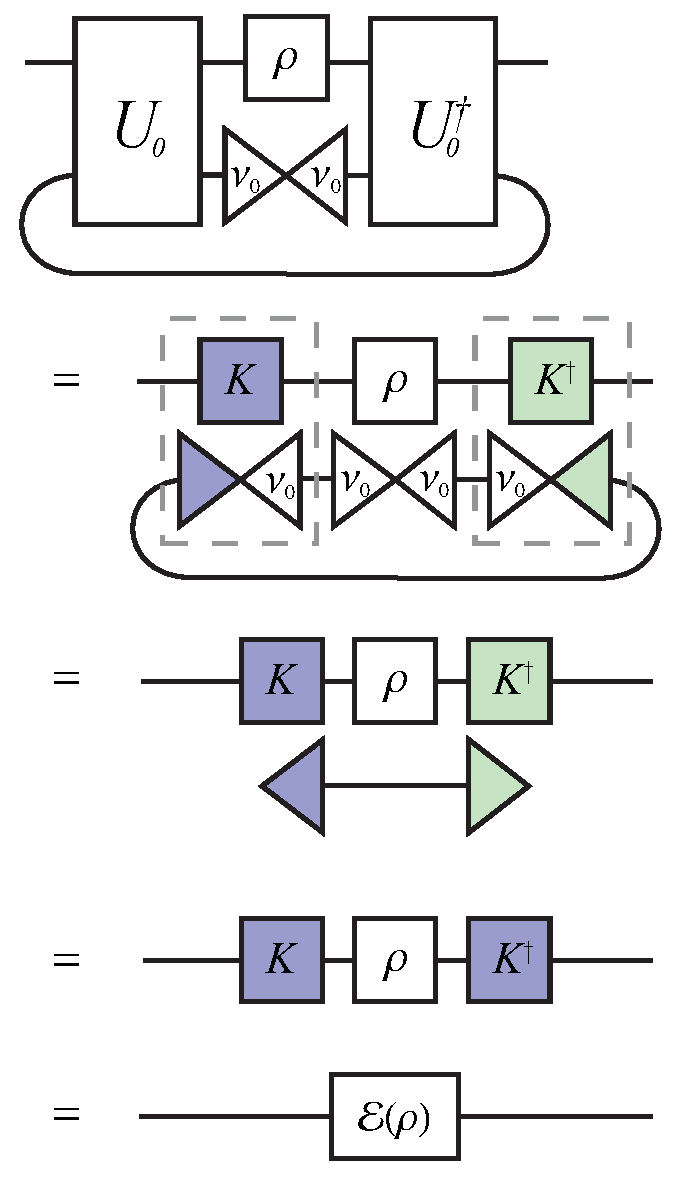
\includegraphics[width=0.33\textwidth]{fig47}
\label{fig:kraus-se-proof}
\end{center}
%
In principle, one may complete the remaining entries of this matrix to construct the full matrix description for the unitary $U$, however such a process is cumbersome and is unnecessary to describe the evolution of the CP-map $\2 E$~\cite{Bengtsson2006}.

We have now finished characterizing the final transformations depicted in Fig.~\ref{fig:cpreps} connecting the Kraus representation to the system-environment representation by Stinespring dilation. As previously mentioned in \S~\ref{sec:to-kraus}, for a fixed choice of basis and initial state for the environment, the transformation between Kraus and Stinespring representations is bijective (and hence so is the transformation between Kraus and system-environment representations when restricted to the subspace spanned by the initial state of the environment). Though both these representations are non-unique, by fixing a basis and initial state for the environment we ensure that this transformation is injective. To see this let $U_0$ and $V_0$ be unitaries restricted to the state $\ket{v_0}$ constructed from Kraus representations, $\{K_\alpha\}$ and $\{J_\alpha\}$ respectively, for $\2 E\in \Cx{X,Y}$. Then 
\begin{eqnarray}
U_0=V_0
&\Leftrightarrow&	\sum_\alpha K_\alpha\otimes\ketbra{\alpha}{v_0} = \sum_\alpha J_\alpha \otimes\ketbra{\alpha}{v_0}\\
&\Leftrightarrow&	\sum_\alpha K_\alpha\braket{\beta}{\alpha} = \sum_\alpha J_\alpha \braket{\beta}{\alpha}\\ 
&\Leftrightarrow& K_\beta = J_\beta
\end{eqnarray}
Bijectivity then follows from the injectivity of the inverse transformation --- the previously given construction of a Kraus representation by the partial trace decomposition of a joint unitary operator in \eqref{fig:kraus-sys-env}. 

%%%%%%%%%%%%%%%%%%%%%%%%%%%%%%%%%%%%%%%%%%%%%%%%%%%%%%%%%%%%

\section{Applications}
\label{sec:ex}

We have now introduced all the basic elements of our graphical calculus for open quantum systems, and shown how it may be used to graphically depict the various representations of CP-maps, and transformations between representations. In this section we move onto more advanced applications of the graphical calculus. We will demonstrate how to apply vectorization to composite quantum systems, and in particular how to compose multiple superoperators together, and construct effective reduced superoperators from tracing out a subsystem. We also demonstrate the superoperator representation of various linear transformations of matrices. These constructions will be necessary for the remaining examples where we derive a succinct condition for a bipartite state to be used for ancilla assisted process tomography, and where we present arguably simpler derivations of the closed form expression for the average gate fidelity and entanglement fidelity of a quantum channel in terms of properties of each of the representations of CP-maps given in \S~\ref{sec:cpmaps}.

%%%%%%%%%%%%%%

\subsection{Vectorization of composite systems}
\label{sec:vec-comp}

We now describe how to deal with vectorization of the general case of composite system of $N$ finite dimensional Hilbert spaces. Let $\2 X_k\cong \C^{d_k}$ be a $d_k$-dimensional complex Hilbert space, and let $\{\ket{i_k}:i_k=0,...,d_k-1\}$ be the standard basis for $\2 X_k$. We are interested in the composite system of $N$ such Hilbert spaces, 
\begin{equation}
\2 X = \2 X_1\otimes...\otimes \2 X_{N}=\bigotimes_{k=1}^{N} \2 X_k
\end{equation}
 which has dimensions $D=\prod_{k=1}^N d_k$. Let $\{\ket{\alpha}: \alpha = 0,..., D-1\}$ be the computational basis for $\2 X$. We can consider vectors in $\2 X$ and the dual space $\2 X^\dagger$ as either 1st-order tensors where their single wire represents an index running over $\alpha$, or as a $N$th-order tensor where each of the $N$ wire corresponds to an individual Hilbert space $\2 X_k$. The correspondence between these two descriptions is made by the concatenation of the composite indices according to the lexicographical order 
 \begin{equation}
 \alpha =\sum_{k=1}^{N} c(k)\, i_k \quad\mbox{where}\quad c(k) := \frac{D}{\prod_{j=1}^k d_j}.
 \end{equation} 
Note that one could also consider the object as any order tensor between 1st and $N$th by the appropriate concatenation of some subset of the wires.

We define the unnormalized Bell-state on the composite system $\XX$ to be the state formed by the column (or row) vectorization of the identity operator $\I_{\2X} \in {\mathcal L}(\2X)$
\begin{eqnarray}
\dket{\I_{\2 X}} 
	&=& \sum_{\alpha=0}^D \ket{\alpha}\otimes\ket{\alpha}\nonumber\\
	&=& \sum_{i_1=0}^{d_1-1}....\sum_{i_N=0}^{d_N-1} \ket{i_1,..., i_N}\otimes\ket{i_1,...,i_N}.
\label{eqn:comp-bell}
\end{eqnarray}
where $\ket{i_1,...,i_N}:=\ket{i_1}\otimes...\otimes\ket{i_N}$. The tensor network for this state is
% FIGURE - MULTI BELL
\begin{center}
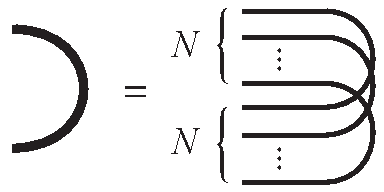
\includegraphics[width=0.25\textwidth]{composite-bell}
\label{fig:composite-bell}    
\end{center}

 
 As with the single system case the column vectorization of a composite linear operator $A \in {\mathcal L}(\2X,\2Y)$, where $\2 Y=\bigotimes_{k=1}^{N} \2 Y_k$,  is given by bending all the system wires upwards, or equivalently by the identity 
 \begin{equation}
 \dket{A}\equiv (\I\otimes A)\dket{\I}.
 \end{equation}
Graphically this is given by
% FIGURE - MULTI VEC
\begin{center}
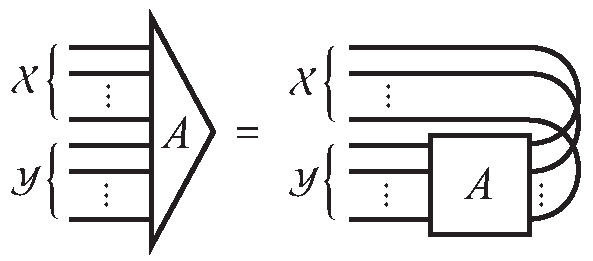
\includegraphics[width=0.45\textwidth]{composite-vec}
\label{fig:composite-vec}
\end{center}
 Note that the order of the subsystems for the bent wires is preserved by the vectorization operation.
 
 % UNRAVELLING
In some situations it may be preferable to consider vectorization of the composite system in terms of vectorization of the individual component systems. Transferring between this component vectorization and the joint-system vectorization can be achieved by an appropriate index permutation of vectorized operators which has a succinct graphical expression when cast in the tensor network framework. 

Suppose the operator $A\in\Lx{X,Y}$, where $\2 X=\bigotimes_{k=1}^N \2 X_k$, $\2 Y=\bigotimes_{k=1}^N \2 Y_k$, is composed of subsystem operators such that 
\begin{equation}
A= A_1\otimes...\otimes A_N
\end{equation} 
where $A_k\in {\mathcal L}(\2 X_k,\2 Y_k)$ for $k=1,...,N$. As previously stated the vectorized composite operator $\dket{A}$ is a vector in the Hilbert space $\XY$. 

We define an operation $\2V_{N}$ called the \emph{unravelling} operation, the action of which unravels a vectorized matrix $\dket{A}= \dket{A_1\otimes\hdots\otimes A_N}$ into the tensor product of vectorized matrices on each individual subsystem $\2 X_k\otimes\2 Y_k$
\begin{equation}
\2V_{N} \dket{A_1\otimes\hdots\otimes A_N}
= \dket{A_1}\otimes\hdots\otimes\dket{A_N} \label{eqn:unravelling}. 
\end{equation}
The inverse operation then undoes the unravelling
\begin{equation}
\2V_{N}^{-1} \big(\dket{A_1}\otimes\hdots\otimes\dket{A_N}\big)
	=\dket{A_1\otimes\hdots\otimes A_n}. 
\end{equation}

More generally the unravelling operation $\2V_{N}$ is given by the map
%
\begin{eqnarray}
\2V_{N}: \ket{x_{\2 X}}\otimes\ket{y_{\2 Y}}
	&\longmapsto& 
	\bigotimes_{k=1}^{N}\left( \ket{x_k}\otimes\ket{y_{k}}\right)
\end{eqnarray}
where 
$\ket{x_{\2 X}} \equiv\ket{x_1}\otimes\hdots\otimes\ket{x_N},
\ket{y_{\2 Y}}\equiv\ket{y_1}\otimes\hdots\otimes\ket{y_N}$.
Hence we can write $\2 V_N$ in matrix form as
\begin{equation}
\2V_N = \sum_{i_1,\hdots,i_{N}}\sum_{j_1,\hdots,j_N} \ket{i_1,j_{1},\hdots,i_N,j_{N}}\bra{i_{\2 X},j_{\2 Y}}.
\label{eqn:unravelling2}
\end{equation}
where $\ket{i_{\2 X}} \equiv\ket{i_1}\otimes\hdots\otimes\ket{i_N},
\ket{j_{\2 Y}}\equiv\ket{j_1}\otimes\hdots\otimes\ket{j_N}$, and $\ket{i_k},\ket{j_l}$ are the standard bases for $\2 X_k$ and $\2 Y_l$ respectively.

We can also express $\2V_N$ as the composition of SWAP operations between two systems. For the previously considered composite operator $A\in {\mathcal L}(\2X,\2Y)$ we have that $\dket{A}$ has $2N$ subsystems. If we label the SWAP operation between two subsystem Hilbert spaces indexed by $k$ and $l$ by $\mbox{SWAP}_{k:l}$, where $1\le k,l\le2N$, then the unravelling operation can be composed as
\begin{equation}
\2V_{N} = W_{N-1}...W_{1}   
\label{eqn:unravelling3}      
\end{equation}
where
\begin{equation}
W_{k} =\prod_{j=0}^{k-1}\,\mbox{SWAP}_{N-k+2j+1:N-k+2j+2}.
\end{equation}
%
For example
\begin{eqnarray}
W_1 &=& \mbox{SWAP}_{N:N+1}\\
W_2 &=& \mbox{SWAP}_{N-1:N}\mbox{SWAP}_{N+1:N+2} \nonumber\\
W_{N-1} &=& \mbox{SWAP}_{2:3}\mbox{SWAP}_{4:5}\hdots \mbox{SWAP}_{2N-2:2N-1}. \nonumber
\end{eqnarray}
While this equation looks complicated, it has a more intuitive construction when depicted graphically. The tensor networks for the unravelling operation in the $N=2,3$ and $4$ cases are shown below
% FIGURE - UNRAVELLING
\begin{center}
 \begin{tabular}{ccc}
 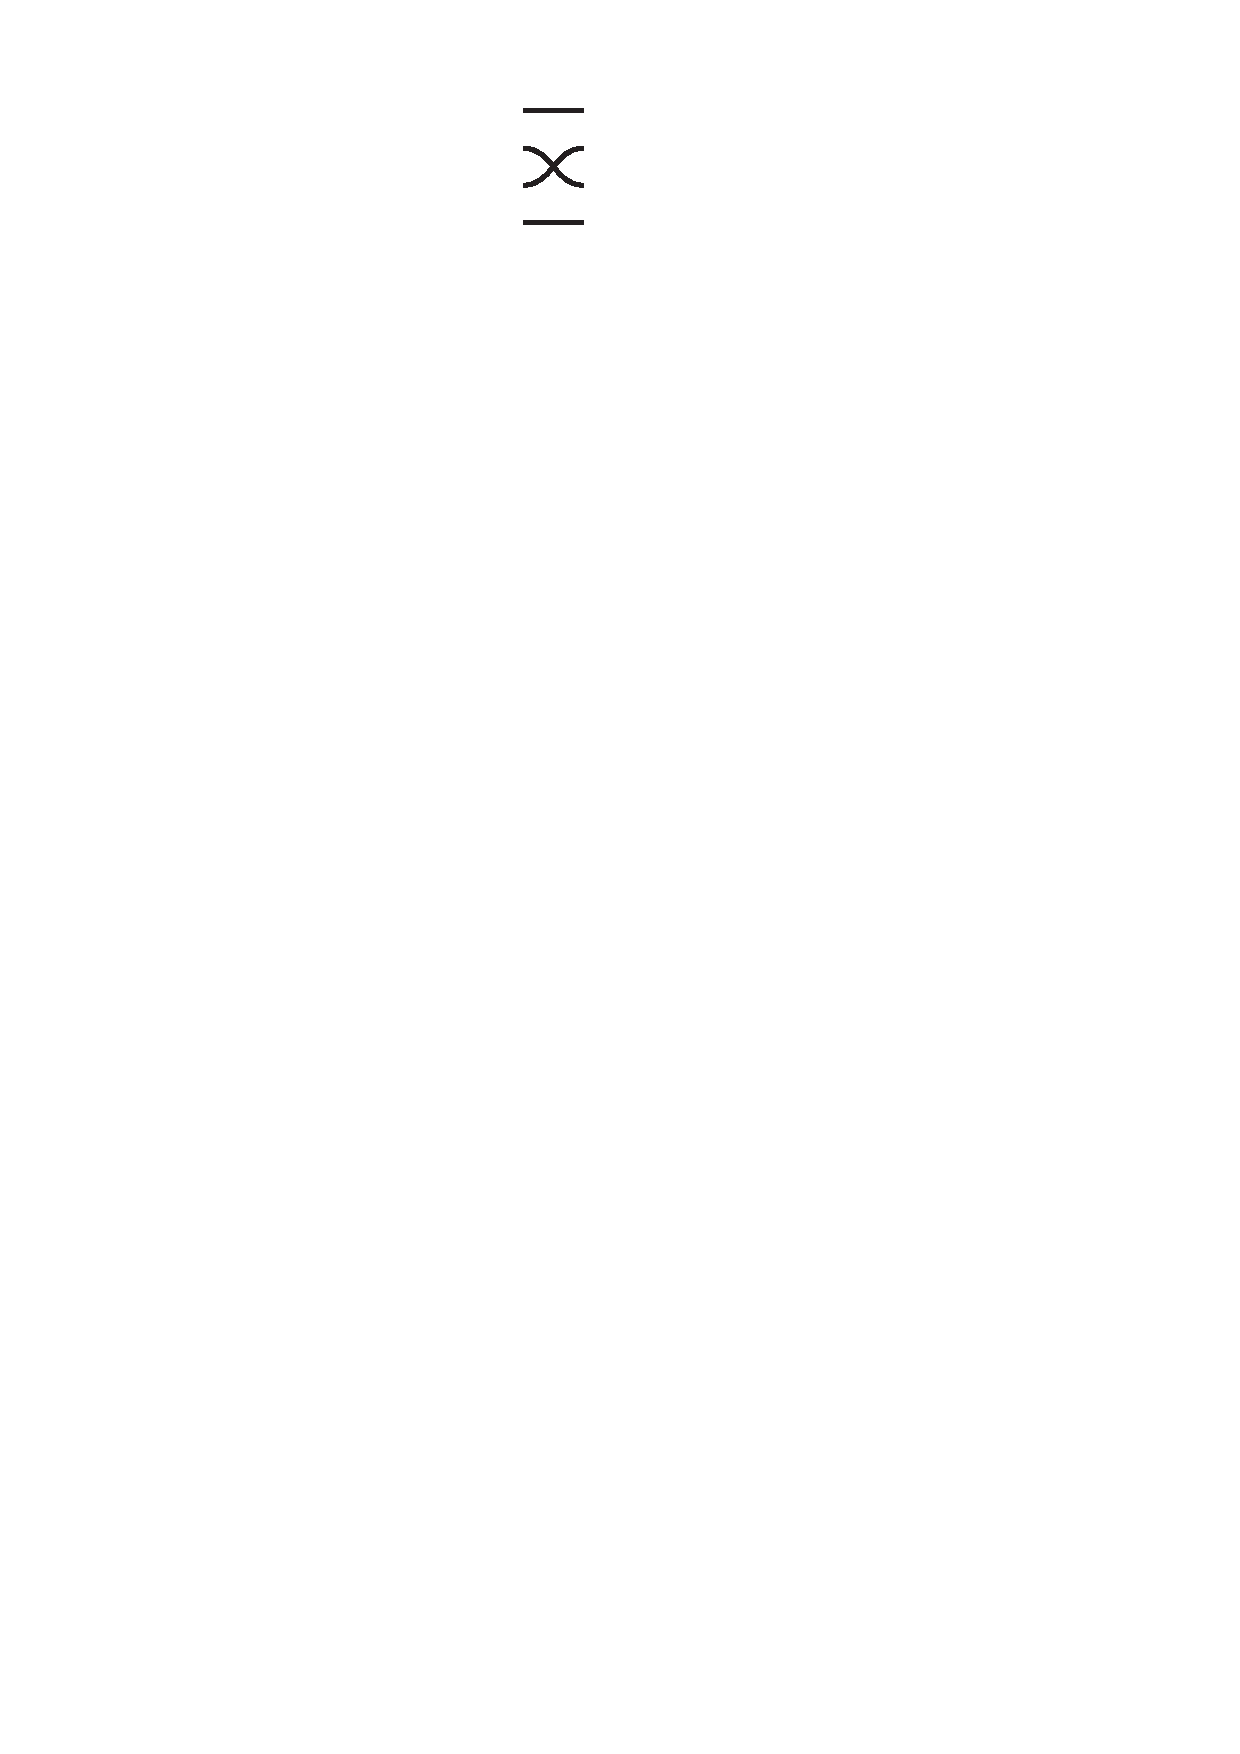
\includegraphics[width=0.07\textwidth]{unravelling-2}
 \quad\quad&\quad\quad
 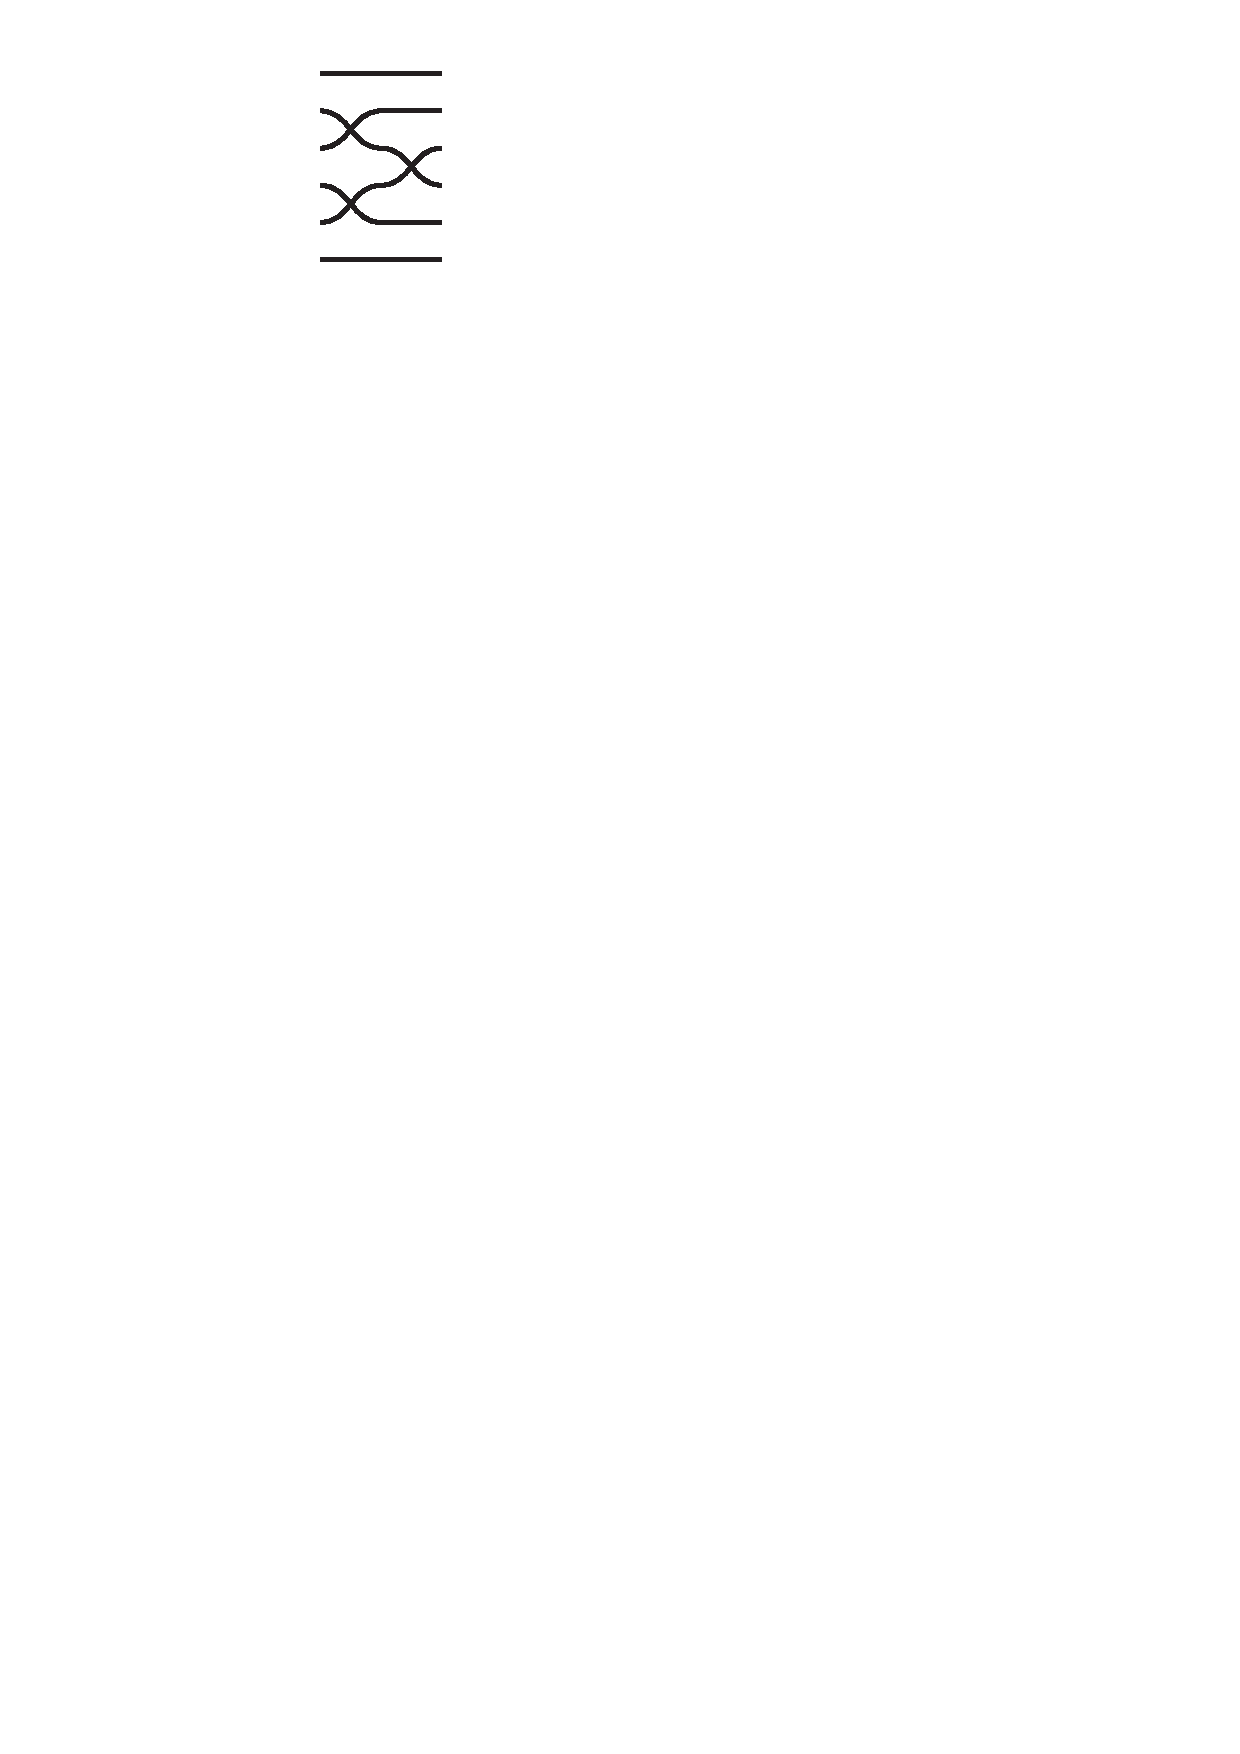
\includegraphics[width=0.1\textwidth]{unravelling-3}
 \quad\quad&\quad\quad
 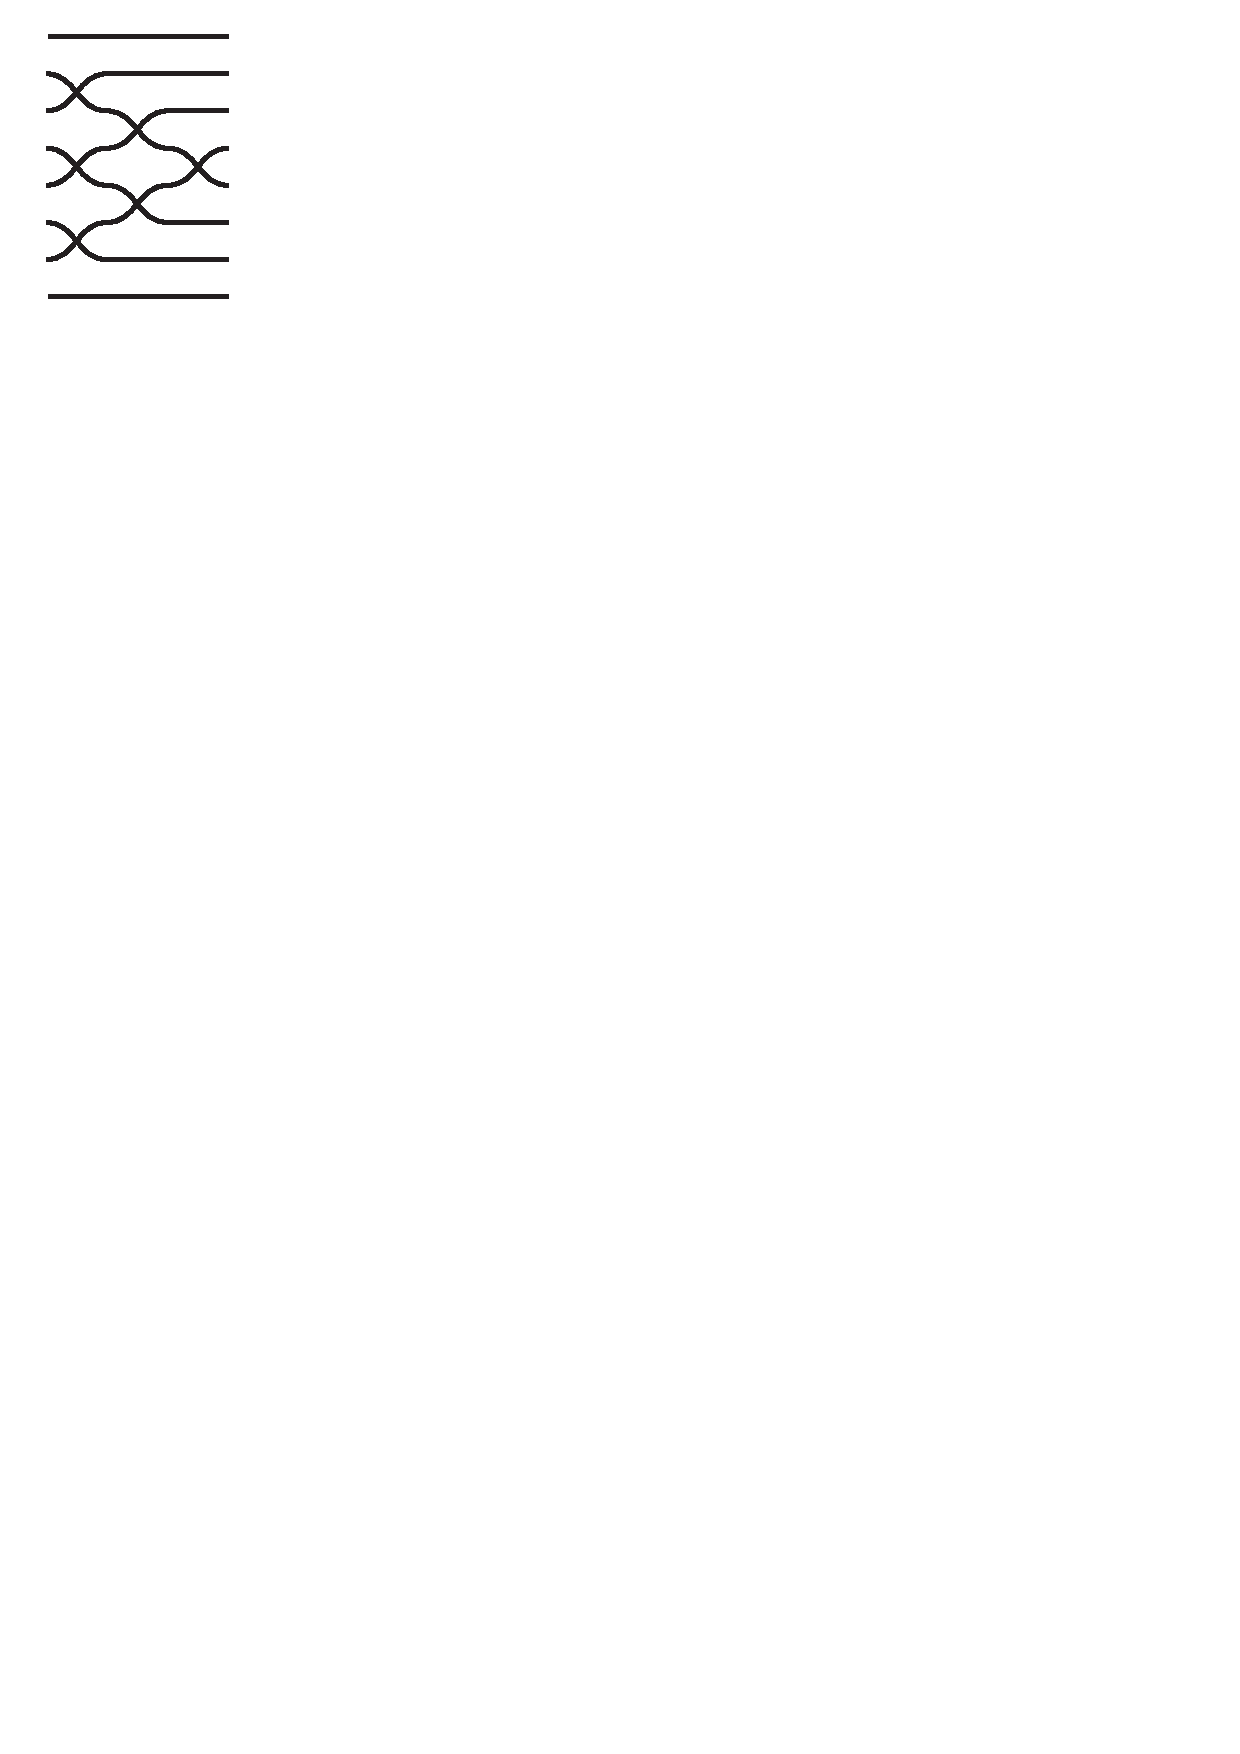
\includegraphics[width=0.13\textwidth]{unravelling-4}
 \\
\footnotesize{(a) $\2V_2$} 
 \quad\quad&\quad\quad
\footnotesize{(a) $\2V_3$} 
  \quad\quad&\quad\quad
  \footnotesize{(a) $\2V_4$} 
 \end{tabular}
  \label{fig:unravelling}
\end{center}
 We also present a graphical proof of this for the $N=3$ case: 
% FIGURE - UNRAVELLING N=3 PROOF
\begin{center}
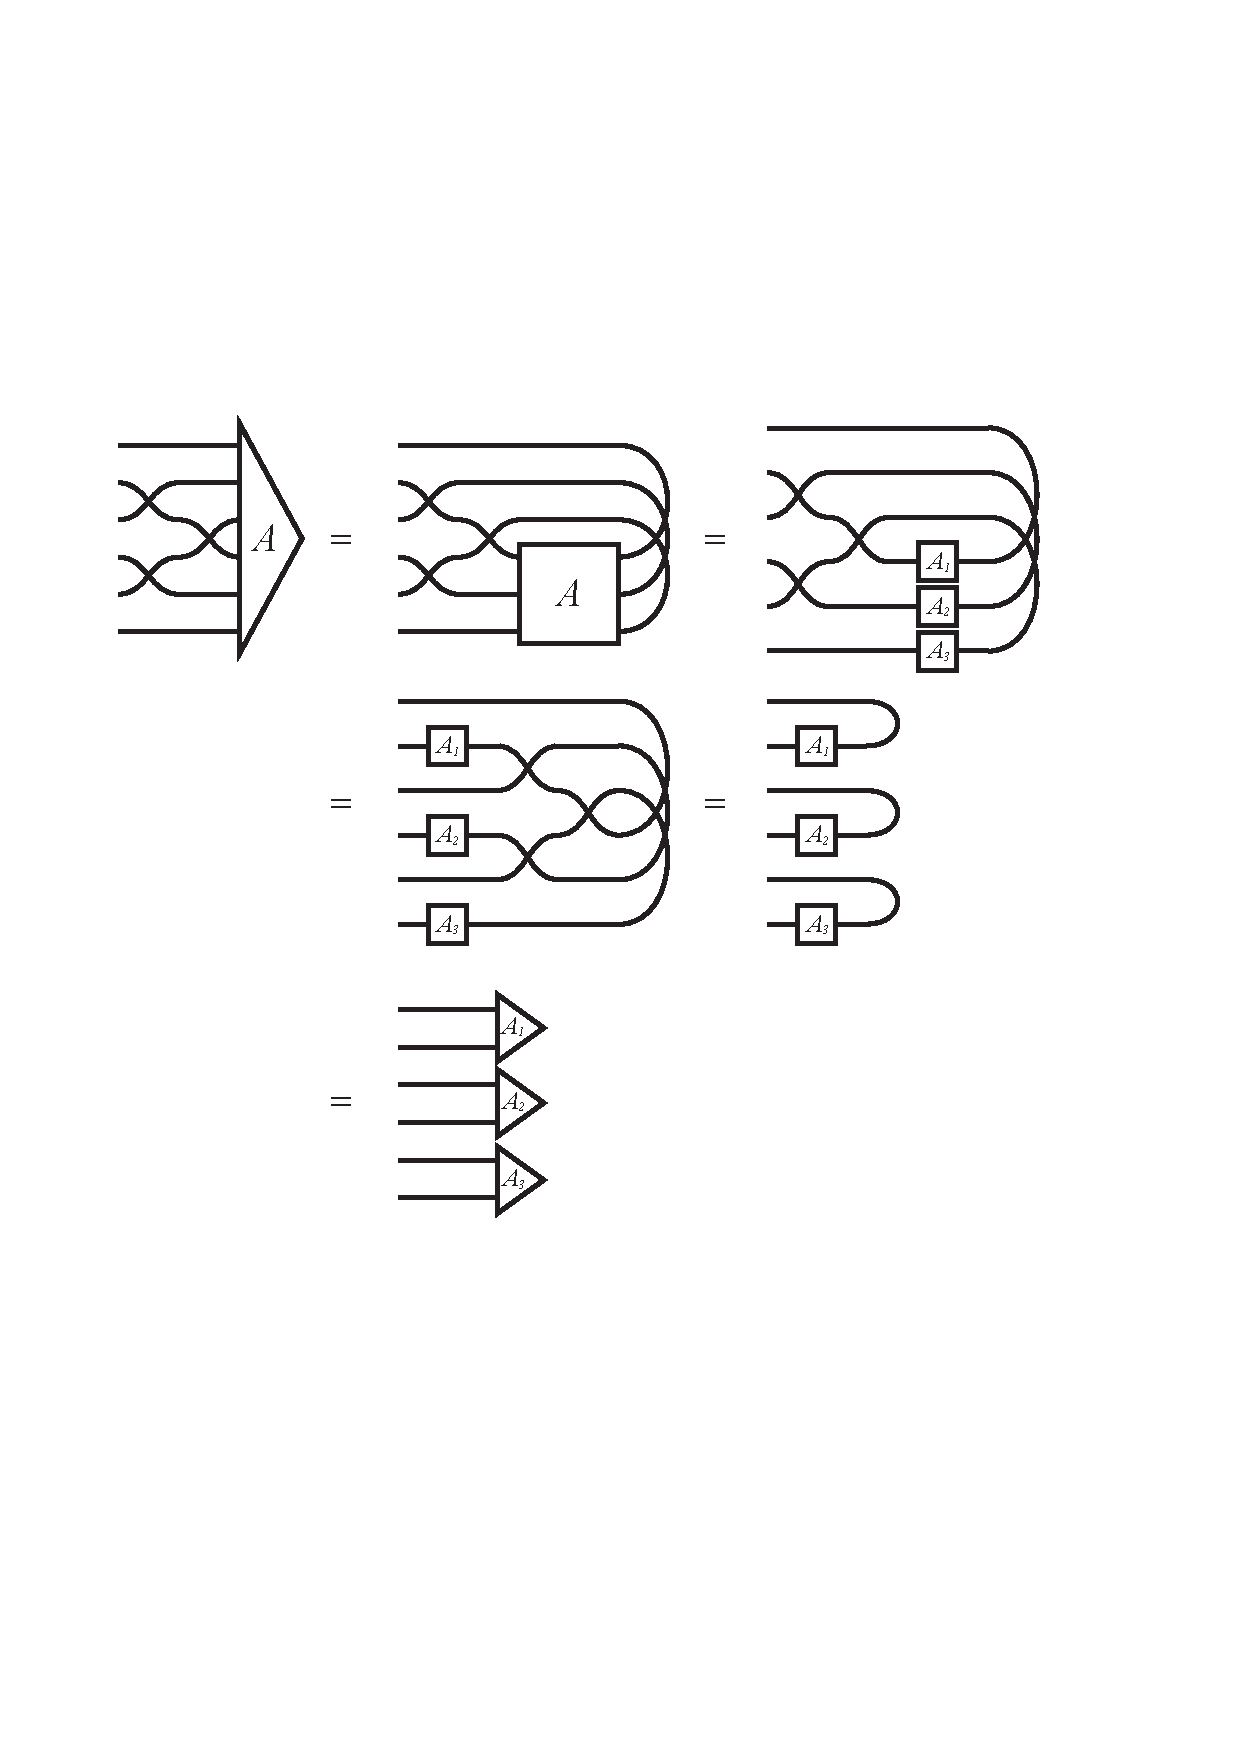
\includegraphics[width=0.5\textwidth]{unravelling-proof}
\label{fig:unravelling-proof}
\end{center}

%%%%%%%%%%%%%%%%%%%%%%%%%%%%%%%%%%%%%%%%%%%%%%%%%%%%%%%%%%%

\subsection{Composing superoperators}
\label{sec:comp-sop}

We now discuss how to compose superoperators on individual subsystems to form the correct superoperator on the composite system, and vice-versa.  Given two superoperators $\2S_1$, and $\2S_2$, if we construct a joint system superoperator via tensor product $(\2S_1\otimes \2S_2)$, this composite operator acts on the tensor product of vectorized inputs $\dket{\rho_1}\otimes\dket{\rho_2}$, rather than the vectorization of the composite input $\dket{\rho_1\otimes\rho_2}$. To construct the correct composite superoperator for input $\dket{\rho_1\otimes\rho_2}$ we may use the unravelling operation $\2V_N$ from \eqref{eqn:unravelling} and its inverse.

If we have a set of superoperators $\{\2S_{k} : k=1,...,N\}$ where $ \2S_k\in {\mathcal L}(\2 X_k\otimes\2X_k,\2Y_k\otimes \2 Y_{k})$, then the joint superoperator $\2 S\in {\mathcal L}(\2X\otimes\2X,\2Y\otimes\2Y)$, where $\2 X=\bigotimes_{k=1}^N \2 X_k$, $\2 Y=\bigotimes_{k=1}^N \2 Y_k$,  is given by
%
\begin{equation}
\2 S = \2 V_N^{\dagger}\left( \2 S_{1}\otimes\hdots\otimes\2 S_{N}\right)\2 V_N.
\label{eqn:comp-sop}
\end{equation} 
The tensor networks for this transformation in the $N=2$ and $N=3$ cases are shown below
% FIGURE - COMPOSE SOP
\begin{center}
\begin{tabular}{c|c}
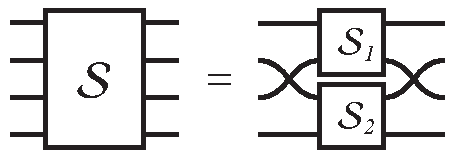
\includegraphics[width=0.3\textwidth]{composite-sop-2}
\quad\quad&\quad\quad
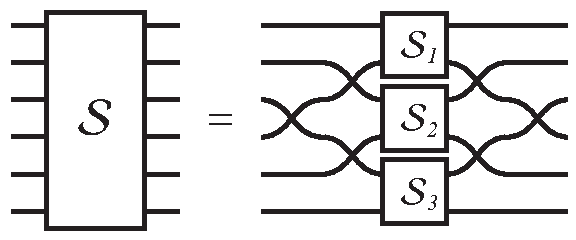
\includegraphics[width=0.38\textwidth]{composite-sop-3}
\\
\footnotesize{$N=2$}
\quad\quad&\quad\quad
\footnotesize{$N=3$}
\end{tabular}
\label{fig:comp-sop}
\end{center}

Composing superoperators from individual subsystem superoperators is useful when performing the same computations for multiple identical systems. For an example we consider vectorization in the Pauli-basis for an $N$-qubit system. While it is generally computationally more efficient to perform vectorization calculations in the col-vec (or row-vec) basis, as these may be implemented using structural operations on arrays, it is often convenient to express the superoperator in the Pauli basis, or the Choi-matrix in the $\chi$-matrix representation, when we are interested in determining the form of correlated errors. However, transforming from the col-vec to the Pauli-basis for multiple (and possibly arbitrary) number of qubits is inconvenient. Using our unravelling operation we can instead compute the single qubit change of basis superoperator $T_{c\rightarrow\sigma}$, where $\sigma=\{\I,X,Y,Z\}/\sqrt{2}$ is the Pauli-basis for a single qubit, and use this to generate the transformation operator for multiple qubits. In the case of $N$-qubits we can construct the basis transformation matrix as
\be
T^{(N)}_{c\rightarrow \sigma} = \2 V_N^{\dagger}\cdot T_{c\rightarrow\sigma}^{\otimes N} \cdot \2 V_N.
\ee
The joint-system superoperator in the Pauli-basis is then given by 
\be
\2 S^\sigma = T^{(N)}_{c\rightarrow \sigma}\cdot\2 S \cdot T^{(N)\dagger}_{c\rightarrow \sigma}
\ee
The same transformation can be used for converting a state $\rho=\rho_1\otimes\hdots\otimes\rho_N$ to the Pauli basis: $\dket{\rho}_\sigma = T^{(N)}_{c\rightarrow \sigma}\dket{\rho}_c$. These unravelling techniques are also useful for applying operations to a limited number of subsystems in a tensor network as used in many tensor network algorithms.

%%%%%%%%%%%%%%%%%%%%%%%%%%%%%%%%%%%%%%%%%%%%%%%%%%

\subsection{Matrix operations as superoperators}
\label{sec:ops-as-sops}

We now show how several common matrix manipulations can be written as superoperators. These expressions are obtained by simply vectorizing the transformed operators. We begin with the trace superoperator $S_{\mbox{\scriptsize{Tr}}}$ which implements the trace of a matrix $S_{\mbox{\scriptsize{Tr}}}\dket{A} := \Tr[A]$ for a square matrix $A\in {\mathcal L}(\2X)$. This operation is simply given by the adjoint of the unnormalized Bell-state:
\be
S_{\mbox{\scriptsize{Tr}}} := \dbra{\I}
\ee
where $\I\in {\mathcal L}(\2X)$ is the identity operator. If $\2X$ is itself a composite system, we simply use the definition of the Bell-state for composite systems from \Eqref{eqn:comp-bell}. This is illustrated in our graphical calculus as
% FIGURE - TRACE
\be
S_{\mbox{\scriptsize{Tr}}}\dket{A} = \parbox[c]{1em}{
\includegraphics[width=0.1\textwidth]{vec-tr}}
\label{fig:vec-tr}
\ee

For a rectangular matrix $B\in {\mathcal L}(\2X,\2Y)$, the transpose superoperator $S_{T}$ which implements the transpose $S_T\dket{B}=\dket{B^T}$ is simply a swap superoperator between $\2X$ and $\2 Y$.
\begin{eqnarray}
S_{T} &=& \mbox{SWAP}	\\
\mbox{SWAP}&:& \XY \mapsto \YX  
\end{eqnarray}
The tensor network for the swap superoperator is 
% FIGURE - TRANS
\be
S_{\mbox{\scriptsize{T}}}\dket{B} = \parbox[c]{0.1\textwidth}{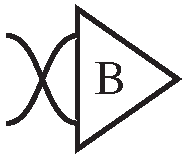
\includegraphics[width=0.1\textwidth]{vec-trans}}
\label{fig:vec-trans}
\ee
If $\2X$ and $\2Y$ are composite vector spaces we may split the crossed wires into their respective subsystem wires. 

Next we give the superoperator representations of the bipartite matrix operations in \eqref{fig:bipartite} acting on vectorized square bipartite matrices $M\in {\mathcal L}(\XY)$. These are the partial trace over $\2X$ ($S_{\mbox{\scriptsize{Tr}}_{\2 X}}$) (and $S_{\mbox{\scriptsize{Tr}}_{\2Y}}$ over $\2 Y$), transposition $S_T$, 
and col-reshuffling $(S_{R_c})$. 
\begin{eqnarray}
S_{\mbox{\scriptsize{Tr}}_{\2 X}}
	&:& \XY\otimes\XY \mapsto \2Y\otimes\2Y\\
S_{\mbox{\scriptsize{Tr}}_{\2 Y}}
	&:& \XY\otimes\XY \mapsto \2X\otimes\2X\\
S_{\mbox{\scriptsize{T}}}
	&:&	 \XY\otimes\XY \mapsto \XY\otimes\XY\\
S_{\scriptsize{R_c}}
	&:&	 \XY\otimes\XY \mapsto \XX\otimes\YY
\end{eqnarray}

\begin{fullpage}
The graphical representation of the superoperators for these operations are:
% FIGURES - BIPARTITE
\begin{center}
\begin{tabular}{c|c|c|c}
$S_{\mbox{\scriptsize{Tr}}_{\2 X}}\dket{M}
=$ \parbox[c]{0.11\textwidth}{
\includegraphics[width=0.09\textwidth]{vec-bi-trx}}
&\quad
$S_{\mbox{\scriptsize{Tr}}_{\2 Y}}\dket{M}
=$ \parbox[c]{0.11\textwidth}{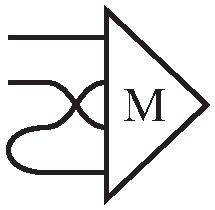
\includegraphics[width=0.09\textwidth]{vec-bi-try}}
&\quad
$S_{\mbox{\scriptsize{T}}}\dket{M}
=$ \parbox[c]{0.11\textwidth}{
\includegraphics[width=0.09\textwidth]{vec-bi-trans}}
&\quad
$S_{\scriptsize{R_c}}\dket{M}
=$ \parbox[c]{0.11\textwidth}{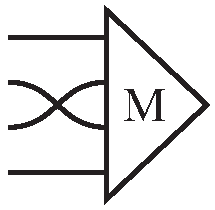
\includegraphics[width=0.09\textwidth]{vec-bi-rc}}
\end{tabular}
\label{fig:bipartite-sop}
\end{center}
\end{fullpage} 

Algebraically they are given by
\begin{eqnarray}
S_{\mbox{\scriptsize{Tr}}_{\2 X}}
	&=&	\big[\dbra{\I_{\2 X}}\otimes\I_{\2 Y}\otimes \I_{\2 Y}\big]\2 V_2\\
S_{\mbox{\scriptsize{Tr}}_{\2 Y}}
	&=&	\big[\I_{\2 X}\otimes \I_{\2 X}\otimes\dbra{\I_{\2 Y}}\big]\2 V_2\\
S_{\mbox{\scriptsize{T}}}
	&=&	\mbox{SWAP}_{1:3}\mbox{SWAP}_{2:4}\\
S_{\scriptsize{R_c}}
	&=&	 \2V_2
\end{eqnarray}
where $\2V_2$ is the unravelling operation in \Eqref{eqn:unravelling}. 

In the general multipartite case for a composite matrix $A\in {\mathcal L}(\2X)$ where $\2 X=\bigotimes_{k=1}^N \2 X_k$, we can trace out or transpose a subsystem $j$ by using the unravelling operation in \Eqref{eqn:unravelling} to insert the appropriate superoperator for that subsystem with identity superoperators on the remaining subsystems:
\begin{eqnarray*}
\2S_{O_j} 
&=& 
	\2 V_{N-1}^{-1}\left[
		\left(\bigotimes_{k=1}^{j-1}\2S_{\2 I_{k}}\right)
		\otimes\2S_{O}\otimes
		\left(\bigotimes_{k=j+1}^{N}\2S_{\2 I_{k}}\right)
	\right]\2 V_N	\\
\end{eqnarray*}
where $\2S_O\in T(\2 X_j)$ is the superoperator acting on system $j$ and $\2S_{\2 I_k}\in T(\2 X_k)$ is the identity superoperator for subsystem $ {\mathcal L}(\2 X_k)$. Similarly by inserting the appropriate operators at multiple subsystem locations we can perform the partial trace or partial transpose of any number of subsystems.

%%%%%%%%%%%%%%%%%%%%%%%%%%%%%%%%%%%%%%%%%%%%%%%%%%%%%%%

\subsection{Reduced superoperators}
\label{sec:reduced-sop}

We now present a simple but useful example of the presented bipartite operations in the superoperator representation to show how to construct an effective reduced superoperator for a subsystem out of a larger superoperator on a composite system.

Consider states $\rho_{XY}\in {\mathcal L}(\XY)$ which undergo some channel $\2 F\in C(\XY)$ with superoperator representation $\2S$. Suppose system $\2Y$ is an ancilla which we initialize in some state $\tau_{0}\in {\mathcal L}(\2Y)$, and we post-select on the output state of system $\2Y$ being in a state $\tau_{1}$. We may construct the effective reduced map $\2 F^\prime\in T(\2X)$ for this process for arbitrary input and output states of system $\2X$, given by a superoperator $\2S^\prime$, as shown:
% FIGURE - REDUCED SOP
\begin{center}
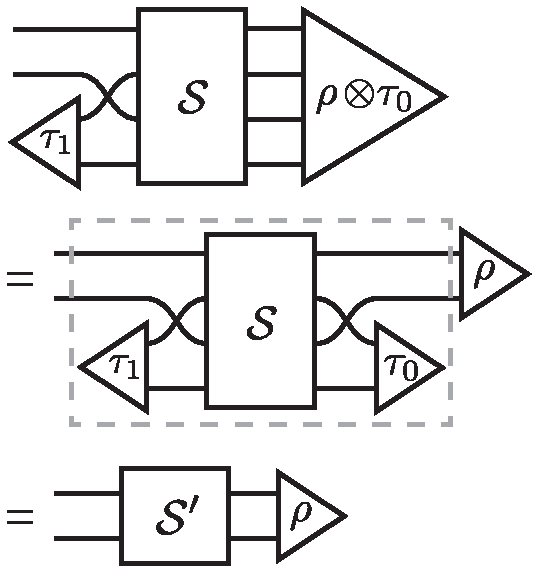
\includegraphics[width=0.35\textwidth]{reduced-sop}
\label{fig:reduced-sop}
\end{center}

Formally, we are defining the superoperator representation $\2S^\prime$ of the effective channel $\2 F^\prime$ as the map
\begin{eqnarray}
\2 F^\prime(\rho) &=& \Tr_{\2 Y}\left[(\I_{\2X}\otimes\tau_1)\2 F(\rho\otimes\tau_0)\right]	\\
\2 S^\prime &=& \dbra{\tau_1}\2V_2 \2S\2V_2^\dagger\dket{\tau_0}
\end{eqnarray} 
where $\2S$ is the superoperator representation of $\2F$ and $\dket{\tau_j}$ is implicitly assumed to have the identity operation on the vectorization of subsystem $\2X\otimes\2X$ $(\dket{\tau_j}:= \I_{\2X}\otimes\I_{\2X}\otimes \dket{\tau_j})$.

%%%%%%%%%%%%%%%%%%%%%%%%%%%%%%%%%%%%%%%%%%%%%%%%%%%%%

\subsection{Ancilla Assisted Process Tomography}
\label{sec:aapt}

Quantum state tomography is the method of reconstructing an unknown quantum state from the measurement statistics obtained by performing a tomographically complete set of measurements on many identical copies of the unknown state~\cite{NC}. Quantum process tomography is an extension of quantum state tomography which reconstructs an unknown quantum channel $\2E\in C(\2X)$ from appropriately generated measurement statistics. One such procedure, known as \emph{standard quantum process tomography}, involves preparing many copies of each of a tomographically complete set of input states, subjecting each to the unknown quantum channel, and performing state tomography on the output~\cite{DAriano2001}. 

An alternative approach is to directly measure the Choi-matrix for the channel via a method known as \emph{ancilla assisted process tomography} (AAPT)~\cite{White2003}. The simplest case of AAPT is \emph{entanglement assisted process tomography}(EAPT) which is an experimental realization of the Choi-Jamio{\l}kowski isomorphism. Here an experimenter prepares a maximally entangled state 
\be
\rho_{\Phi}= \frac{1}{d}\dketdbra{\I}{\I}
\ee 
across the system of interest $\2X$ and an ancilla $\2Z \cong \2X$, and subjects the system to the unknown channel $\2E$, and the ancilla to an identity channel $\2I$. The output of this joint system-ancilla channel is the rescaled Choi-matrix:
\begin{eqnarray}
\rho_{\phi}^\prime = (\2I\otimes\2E)\left(\rho_{\Phi}\right) 
	&=& \frac{\Lambda}{d}.
\end{eqnarray}
which can be measured directly by quantum state tomography. The tensor network for EAPT is
% FIGURE - EAPT
\begin{center}
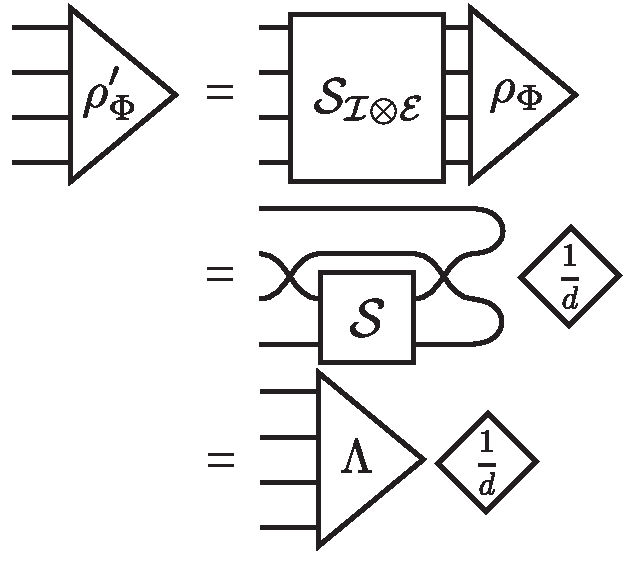
\includegraphics[width=0.4\textwidth]{app-aapt-choi}
\label{fig:aapt-choi}
\end{center}

In general AAPT does not require $\rho_{AS}$ to be maximally entangled. It has been demonstrated experimentally that AAPT may be done with a state which does not have any entanglement at all, at the expense of an increase in the estimation error of the reconstructed channel~\cite{White2003}. A necessary and sufficient condition for a general state $\rho_{AS}$ to allow recovery of the Choi-matrix of an unknown channel $\2E$ via AAPT is that it have a \emph{Schmidt number} equal to $d^2$ where $d$ is the dimension of the state space $\2X$~\cite{White2003}. This conditions has previously been called \emph{faithfulness} of the input state, and one can recover the original Choi-matrix for the unknown channel $\2E$ by applying an appropriate inverse map to the output state in post-processing~\cite{DAriano2003}. We provide an arguably simpler derivation of this condition, and the explicit construction of the inverse recovery operator. The essence of this proof is that we can consider the bipartite state $\rho_{AS}$ to be Choi-matrix for an effective channel via the Choi-Jamio{\l}kowski isomorphism (but with trace normalization of 1 instead of $d$) . We can then apply channel transformations to this initial state to convert it into an effective channel acting on the true Choi-matrix, and if this effective channel is invertible we can recover the Choi-matrix for the channel $\2E$ by applying the appropriate inverse channel.

% PROPOSITION
\begin{proposition}
\label{prop:aapt}
$(a)$ A state $\rho_{AS}\in {\mathcal L}(\2X\otimes\2X)$ may be used for AAPT of an unknown channel $\2E\in  C(\2X)$ if and only if the reshuffled density matrix $\2S_{AS} = \rho_{AS}^{R_c}$ is invertible. 

$(b)$ The channel can be reconstructed from the measured output state by $\Lambda_{\2E} = (\2R\otimes \2I)(\rho_{AS}^\prime)$
where $\rho_{AS}^\prime = (\2 I\otimes \2E)(\rho_{AS})$ is the output state reconstructed by quantum state tomography, and $\2R$ is the recovery map given by superoperator $\2S_{\2R} = (\2S_{AS}^T)^{-1}$.
\end{proposition}

The graphical proof of Prop.~\ref{prop:aapt}  is illustrated in Fig.~\ref{fig:aapt-proof}. This proof demonstrates several useful features of the presented graphical calculus. In particular it applies the vectorized reshuffling transformation to a bipartite density matrix input state to obtain an effective superoperator representation of a state, and uses the unravelling operation for composition of superoperators.
From this construction we find that if the initial state $\rho_{AS}$ is maximally entangled, then it can be expressed as $\rho_{AS}= \dketdbra{V}{V}$ for some unitary $V$. In this case the reshuffled superoperator of the state corresponds to a unitary channel $\2S_{AS} = \overline{V}\otimes V$, and hence is invertible with $\2S_{AS}^{-1} = \2S_{AS}^\dagger$. If the input state is not maximally entangled, then the closer it is to a singular matrix, the larger the condition number and hence the larger the amplification in error when inverting the matrix.

% FIGURE - AAPT GRAPHICAL PROOF
\begin{figure}[ht]
\centering
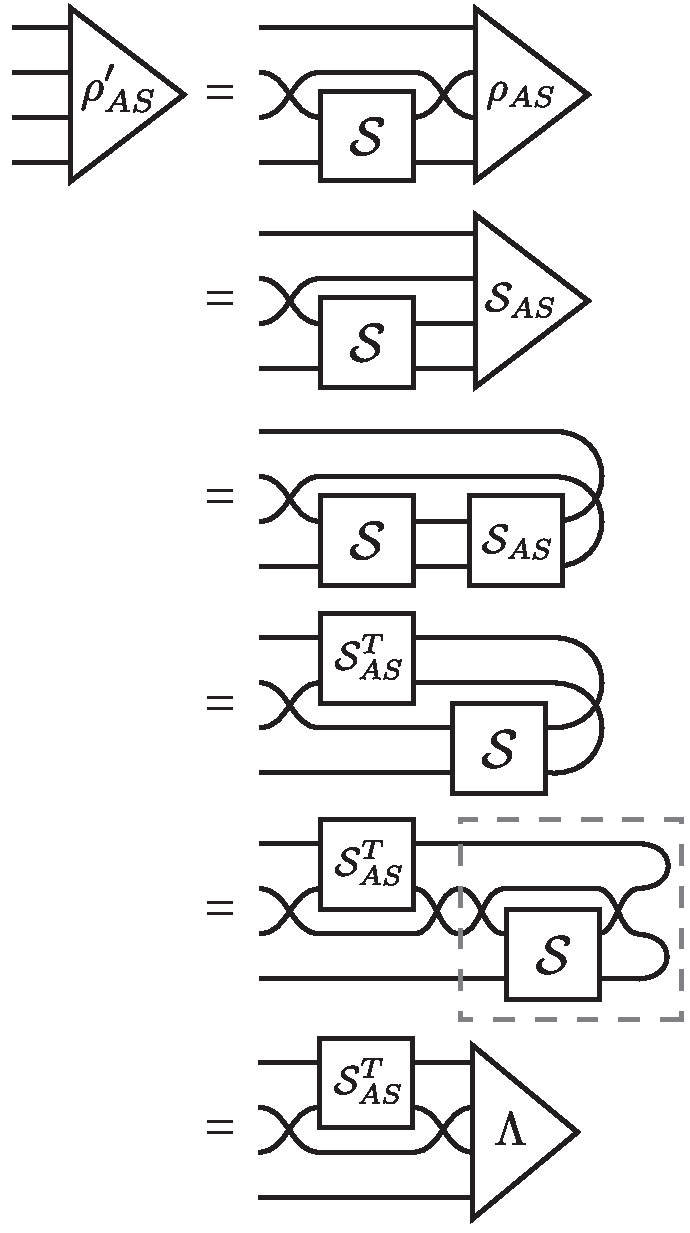
\includegraphics[width=0.4\textwidth]{app-aapt-proof}
\caption{Graphical proof of the equivalence of an initial state $\rho_{AS}$ used for performing AAPT of an unknown CPTP map $\2E$ with superoperator representation $\2S$, to a channel $(\2R\otimes\2I)$ acting on the Choi-matrix $\Lambda$ for a channel $\2E$. The Choi-matrix can be recovered if and only if the superoperator $\2S_{\2R}=\2S_{AS}^T=(\rho_{AS}^{R_c})^T$ is invertible.}
\label{fig:aapt-proof}
\end{figure}

%%%%%%%%%%%%%%%%%%%%%%%%%%%%%%%%%%%%%%%%%%%%%%%%%%

\subsection{Average Gate Fidelity}
\label{sec:gatefid}

When characterizing the performance of a noisy quantum channels a widely used measure of the closeness of a CPTP map $\2E\in C(\2X)$ to a desired quantum channel $\2F\in C(\2X)$ is the \emph{Gate Fidelity}. This is defined to be
\be
F_{\2E,\2F}(\rho) = F(\2F(\rho)\2E(\rho))
\ee
where
\be
F(\rho,\sigma)=\left(\Tr\left[ \sqrt{\sqrt{\rho}\sigma\sqrt{\rho}}\right]\right)^2
\ee
is the fidelity function for quantum states~\cite{NC}.

In general we are interested in comparing a channel $\2E$ to a unitary map $\2U\in C(\2X)$ where $\2U(\rho)=U\rho U^\dagger$. In this case we have
\begin{eqnarray}
F_{\2E,\2U}(\rho) 
	&=& \left[\Tr\sqrt{\sqrt{U\rho U^\dagger}\2E(\rho)\sqrt{U\rho U^\dagger}}\right]^2\\
	&=&  \left[\Tr\sqrt{\sqrt{\rho}U^\dagger\2E(\rho)U\sqrt{\rho}}\right]^2\\
	&=&  \left[\Tr\sqrt{\sqrt{\rho}\,\2U^\dagger(\2E(\rho))\sqrt{\rho}}\right]^2\\
	&=& F_{\2U^\dagger\2E,\2 I}(\rho)
\end{eqnarray}
where $\2I$ is the identity channel and $\2U^\dagger(\rho) = U^\dagger \rho U$, is the adjoint channel of the unitary channel $\2U$. Thus without loss of generality we may consider the gate fidelity $F_{\2E}(\rho)\equiv F_{\2U^\dagger\2F,\2I}(\rho)$ comparing $\2E$ to the identity channel, where we simply define $\2E \equiv \2U^\dagger\2F$ if we wish to compare $\2F$ to a target unitary channel $\2U$.

The most often used quantity derived from the gate fidelity is the \emph{average gate fidelity} taken by averaging $F_{\2E}(\rho)$ over the Fubini-Study measure. Explicitly the average gate fidelity is defined by
\be
\overline{F}_{\2E} = \int d\,\psi\, \bra{\psi} \2E(\ketbra\psi\psi)\ket{\psi}.
\label{eq:avegf}
\ee
where due to the concavity of quantum states we need only integrate over pure states $F_{\2E}(\ketbra\psi\psi) = \bra\psi \2E(\ketbra\psi\psi)\ket\psi$. 

Average gate fidelity is a widely used figure of merit in part because it is simple to compute. The expression in \eqref{eq:avegf} reduces to explicit expression for $\overline{F}_{\2E}$ in terms of a single parameter of the channel $\2E$ itself. This has previously been given in terms of the Kraus representation~\cite{Horodecki1999,Nielsen2002}, superoperator~\cite{Emerson2005} and Choi-matrix in~\cite{Johnston2011}. We now present an equivalent graphical derivation of the average gate fidelity in terms of the Choi-matrix which we believe is simpler than previous derivations. We start with the tensor network diagram corresponding to \eqref{eq:avegf} and perform graphical manipulations as follows
% AVE GATE FIDELITY GRAPHICAL PROOF PT 1
\begin{center}
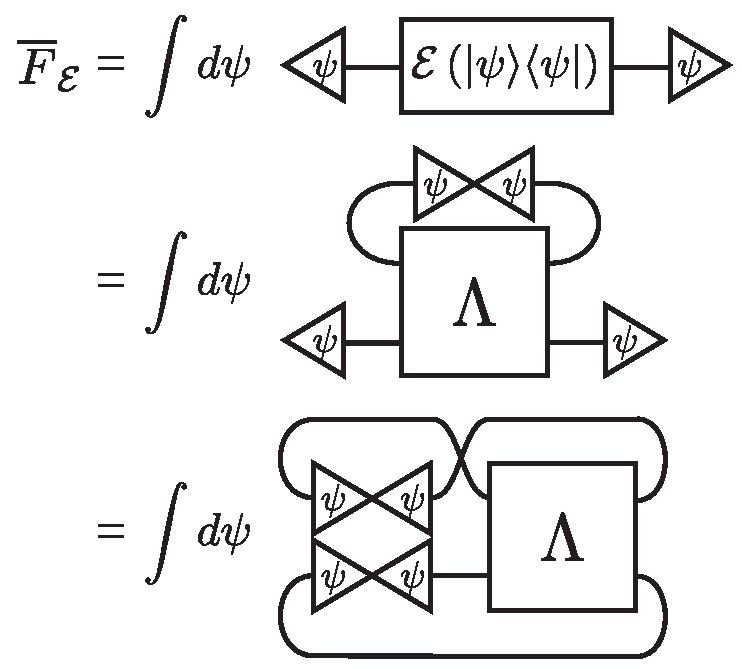
\includegraphics[width=0.35\textwidth]{app-ave-fid-proof-1}
\label{fig:ave-fid-proof-1}
\end{center}
For the next step of the proof we use the result that the average over $\psi$ of a tensor product of states $\ketbra{\psi}{\psi}^n$ is given by
\be
\int d\psi\, \ketbra\psi\psi^{\otimes n} = \frac{\Pi_{\scriptsize\mbox{sym}}(n,d)}{\Tr[\Pi_{\scriptsize\mbox{sym}}(n,d)]}
\label{eq:symsub}
\ee
where $ \Pi_{\scriptsize\mbox{sym}}(n,d)$ is the projector onto the symmetric subspace of $\2X^{\otimes n}$. This projector may be written as~\cite{Magesan2011}
\be
\Pi_{\scriptsize\mbox{sym}}(n,d) = \frac{1}{n!}\sum_\sigma P_{\sigma}
\label{eq:perm-sum}
\ee
where $P_{\sigma}$ are operators for the permutation $\sigma$ of $n$-indices. These permutations may be represented as a swap type operator with $n$ tensor wires. For the case of $n=2$ we have the tensor diagram:
% FIG: SYM SUB
\begin{center}
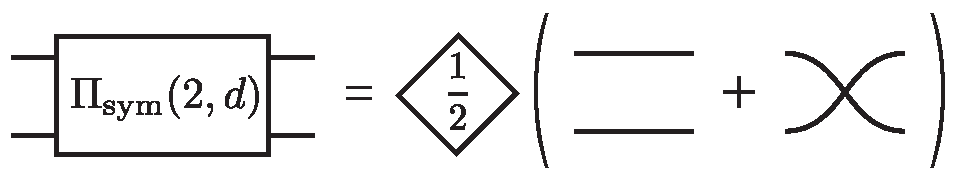
\includegraphics[width=0.45\textwidth]{app-sym-sub-2}
\label{fig:symsub2}
\end{center}
Here we can see that $\Tr[\Pi_{\scriptsize\mbox{sum}}(2,d)] = (d^2 + d)/2$, and hence we have that
\begin{eqnarray}
\Pi_{\scriptsize\mbox{sym}}(2,d) &=& \frac{1}{2}\left(\I\otimes\I + \mbox{SWAP}\right)	\\
\Tr[\Pi_{\scriptsize\mbox{sym}}(2,d)] &=& \frac{d^2+d}{2}	\\
\Rightarrow
\int d\psi\, \ketbra\psi\psi^2 &=& \frac{\I\otimes\I + \mbox{SWAP}}{d(d+1)}
\end{eqnarray}
where $\2X\cong \C^d$, $\I\in {\mathcal L}(\2X)$ is the identity operator, and SWAP is the SWAP operation on $\XX$. Subsituting \eqref{fig:symsub2} into \eqref{fig:ave-fid-proof-1} completes the proof:
% AVE GATE FIDELITY GRAPHICAL PROOF PT 2
\begin{center}
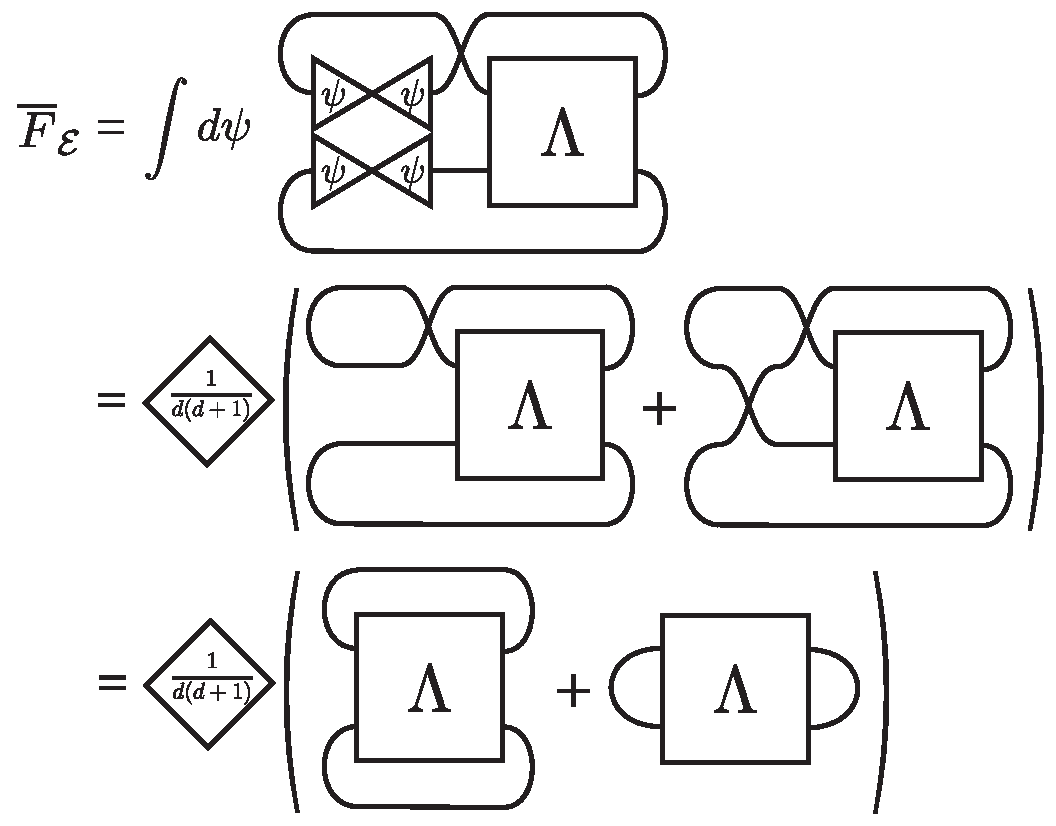
\includegraphics[width=0.48\textwidth]{app-ave-fid-proof-2}
\label{fig:ave-fid-proof-2}
\end{center}
Hence we have that the average gate fidelity in terms of the Choi-matrix is given by
\be
\overline{F}_{\2E} = \frac{d + \dbra{\I}\Lambda\dket{\I}}{d(d+1)}
\ee
where we have used the fact that the Choi-matrix is normalized such that$\Tr[\Lambda] = d$.
From this proof one may derive expressions for the other representations using the channel transformations in \S~\ref{sec:trans}. The resulting expressions are
\begin{eqnarray}
\overline{F}_{\2E} 
	&=& \frac{d + \Tr[\2S]}{d(d+1)}	\\
	&=& \frac{d + \dbra{\I}\Lambda\dket{\I}}{d(d+1)}	\\
	&=& \frac{d + \sum_j |\Tr[K_j]|^2}{d(d+1)}		\\
	&=& \frac{d + d\chi_{00}}{d(d+1)}		\\
	&=& \frac{d + \Tr_{\2X}[A^\dagger]\cdot\Tr_{\2X}[A]}{d(d+1)}
\end{eqnarray}
where $\2S$, $\Lambda$, $\{K_j\}$, $\chi$, $A$ are the superoperator, Choi-matrix, Kraus, $\chi$-matrix and Strinespring representations for $\2E$ respectively. In the case of the $\chi$-matrix representation, $\chi$ is defined with respect to a basis $\{\sigma_j\}$ satisfying $\Tr[\sigma_j] = \sqrt{d}\delta_{j,0}$.

Similar techniques can be applied for tensor networks that may be graphically manipulated into containing a term $\int d\psi\, \ketbra\psi\psi^{\otimes n} $ for $n>2$. This could prove useful for computing higher order moments of fidelity functions and other quantities defined in terms of averages over quantum states $\ket\psi$. In this case there are $n!$ permutations of the tensor wires for the permutation operator $P_\sigma$ in \eqref{eq:perm-sum}, and these can be decomposed as a series of SWAP gates. For example, in the case of $n=3$ we have
\begin{eqnarray}
\Pi_{\scriptsize\mbox{sym}}(3,d) 
&=& \frac{1}{6}\big(
\I^{\otimes 3} + \mbox{SWAP}_{1:2} 
+ \mbox{SWAP}_{1:3}
+ \mbox{SWAP}_{2:3}\\\nonumber 
&+& \mbox{SWAP}_{1:2}\mbox{SWAP}_{2:3}
+ \mbox{SWAP}_{2:3}\mbox{SWAP}_{1:2}\big) 
\end{eqnarray}

\begin{equation}
\Tr[\Pi_{\scriptsize\mbox{sym}}(3,d)] = \frac{d^3+3d^2+2d}{6}.
\end{equation}

%%%%%%%%%%%%%%%%%%%%%%%%%%%%%%%%%%%%%%%%%%%%%%%%%%%%%%

\subsection{Entanglement Fidelity}
\label{sec:entfid}

Another useful fidelity quantity is the \emph{entanglement fidelity} which quantifies how well a channel preserves entanglement with an ancilla~\cite{Schumarcher1996,NC}. For a CPTP map $\2E\in C(\2X)$ and density matrix $\rho\in {\mathcal L}(\2X)$ the entanglement fidelity is given by 
\begin{eqnarray}
F_{\scriptsize\mbox{e}}(\2E,\rho) 
&=& \inf
	\big\{
	F\left(\ketbra{\psi}{\psi}, (\2I_{\2Z}\otimes\2E)(\ketbra{\psi}{\psi})\right):
\nonumber\\&&
	\Tr_{\2Z}[\ketbra{\psi}{\psi}]=\rho \big\}
\label{eq:ent-fid}
\end{eqnarray}
where $\ket\psi\in \2X\otimes\2Z$ is a purification of $\rho$ over an ancilla $\2Z$. Entanglement fidelity turns out to be independent of the choice of purification $\ket\psi$, and a closed form expression has been given in terms of the Kraus representation~\cite{NC} and Choi-matrix~\cite{Fletcher2007}. Here we present a simple equivalent derivation in terms of the Choi-matrix representation of the channel $\2E$ using graphical techniques. Then by applying the channel transformations of \S~\ref{sec:trans} we obtain expressions in terms of the other representations. The resulting expressions for entanglement fidelity are:
\begin{eqnarray}
F_{\scriptsize\mbox{e}}(\2E,\rho) 
	&=& \dbra{\rho}\Lambda\dket{\rho}	\\
	&=& \Tr\left[(\rho^T\otimes\rho)\2S\right]	\\
	&=& \sum_j |\Tr[\rho K_j]|^2 \\
	&=& \sum_{i,j}\chi_{ij} \Tr[\rho\, \sigma_i]\Tr[\rho \sigma^\dagger_j]\\
	&=&\Tr_{\2X}[\rho A^\dagger]\cdot\Tr_{\2X}[A\rho]
\end{eqnarray}
where $\2S$, $\Lambda$, $\{K_j\}$, $\chi$, $A$ are the superoperator, Choi-matrix, Kraus, $\chi$-matrix and Strinespring representations for $\2E$ respectively. In the case of the $\chi$-matrix representation, $\chi$ is defined with respect to a basis $\{\sigma_j\}$ satisfying $\Tr[\sigma_j] = \sqrt{d}\delta_{j,0}$. 

For the graphical proof in terms of the Choi-representation we start with \eqref{eq:ent-fid} and perform the following tensor manipulations
% ENTANGLEMENT FIDELITY GRAPHICAL PROOF - 1 
\begin{center}
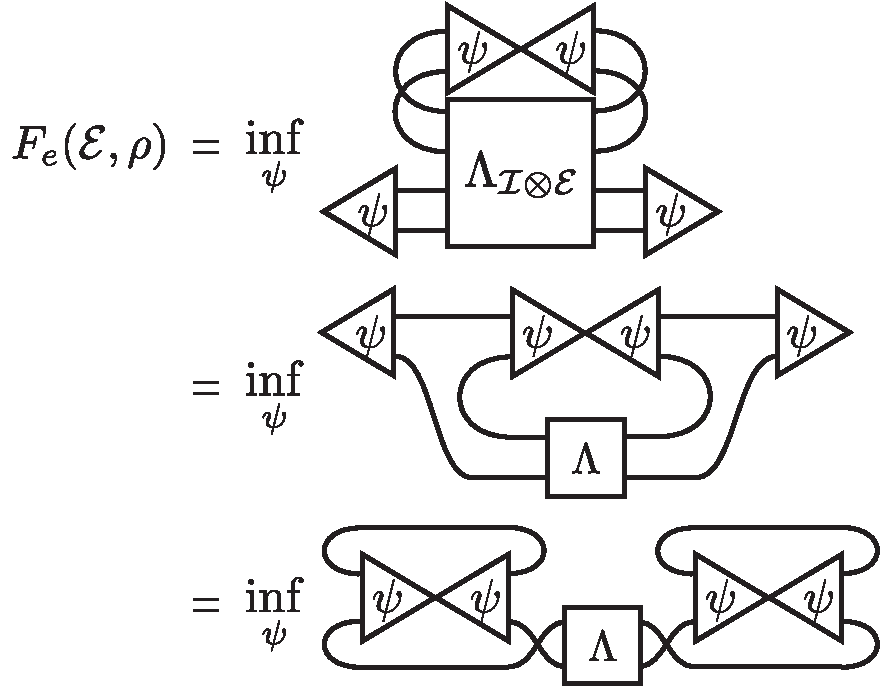
\includegraphics[width=0.45\textwidth]{app-ent-fid-proof-1}
\label{fig:ent-fid-proof-1}
\end{center}
Now since the infimum is over all $\ket{\psi}\in \2Z\otimes\2X$ satisfying $\Tr_{\2Z}[\ketbra{\psi}{\psi}]=\rho$ the result is independent of the specific purification $\psi$ and we have:
% ENTANGLEMENT FIDELITY GRAPHICAL PROOF - 2 
\begin{center}
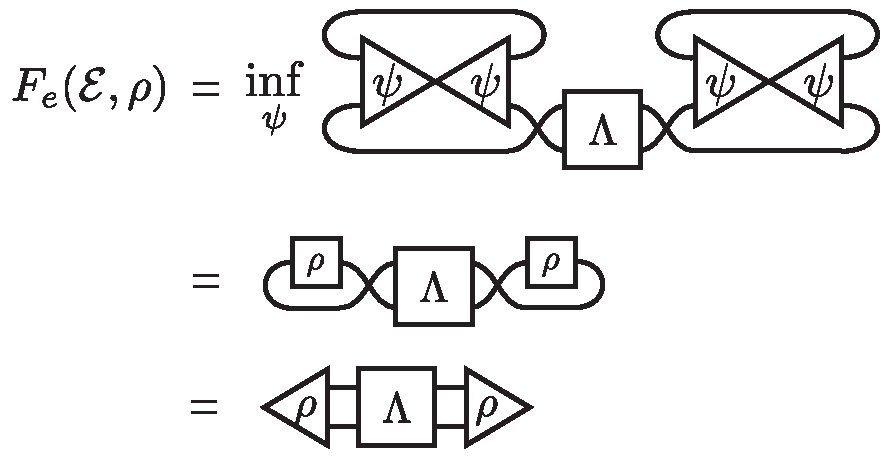
\includegraphics[width=0.45\textwidth]{app-ent-fid-proof-2}
\label{fig:ent-fid-proof-2}
\end{center}

Entanglement fidelity is equivalent to gate fidelity for pure states and hence average entanglement fidelity is equivalent to average gate fidelity. This can be shown graphically as follows
% ENTANGLEMENT FIDELITY REPS PROOF
\begin{center}
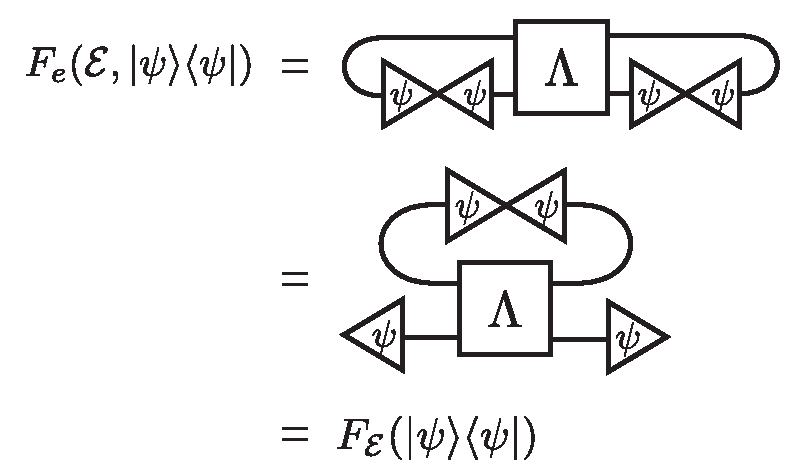
\includegraphics[width=0.45\textwidth]{app-ent-gate-proof}
\label{fig:ent-gate-proof}
\end{center}
Alternatively we can also define the average gate fidelity in terms of the entanglement fidelity with the identity operator
\be
\overline{F}_{\2E} = \frac{d + F_e(\2E, \I)}{d(d+1)}.
\ee

\section{Further Studies}

Open quantum systems represents an active and poorly understood area of research with results appearing frequently.  

Further directions include and are not limited to. 
% PS
%\begin{enumerate}
\begin{itemize}
    \item[1.] % PS 
    Present a tensor network explanation for entanglement breaking channels---see Figure 1 in \cite{Filippov_2013}.  (suggested by Sergey Filippov) 
    \item[2.] %PS
     Extending open dynamics to  non-Markovianity by considering the process tensor which corresponds to a recent debate in the community \cite{Milz_2017} see also Figure 1 \cite{luchnikov2019machine}. (suggested by Kavan Modi and then Sergey Filippov) 
    
    \item[3.]%PS
     Extend ideas related to \eqref{eqn:choithm}. $\2 E$ is unital iff $\Tr_{\2 X}[\Lambda]=\I_{\2 Y}$.  According to Konstantin Antipin, an interesting tensor network corresponds to that too---similar to \eqref{eqn:choi-TP}. (suggested by Konstantin Antipin and then Sergey Filippov) 
%\end{enumerate}
\end{itemize} % PS, test




